\documentclass[11pt,a4paper,twoside,openany]{report}
\usepackage[T1]{fontenc}
\usepackage[utf8]{inputenc}
\usepackage{lmodern}
\usepackage[margin=25mm]{geometry}
\usepackage{graphicx}
\usepackage{booktabs}
\usepackage{longtable}
\usepackage{array}
\usepackage{amsmath}
\usepackage{microtype}
\usepackage{setspace}

\usepackage[numbers,sort&compress]{natbib}
\usepackage{xcolor}
\usepackage[hidelinks]{hyperref}
\usepackage{caption}
\captionsetup{font=small,labelfont=bf}
\graphicspath{{figures/}}
\setlength{\parskip}{4pt}
\onehalfspacing
\newcommand{\claim}[1]{\textbf{[#1]}}
\newcommand{\resfile}[1]{\texttt{\small #1}}

\title{Histology-anchored multimodal deep learning in oesophageal cancer:\\
where and why fusion fails to replicate, and how to validate report-derived supervision}
\author{Rehan Zuberi\\[4pt]
\normalsize Cancer Research UK Cambridge Institute\\
\normalsize University of Cambridge}
\date{Working draft, 15 September 2026}

\begin{document}
\maketitle
\chapter*{Abstract}
\addcontentsline{toc}{chapter}{Abstract}

Multimodal deep learning models that combine haematoxylin-and-eosin (H\&E) histology with genomic or clinical data are widely reported to outperform histology alone. This thesis asks whether that advantage replicates in oesophageal cancer and its precursor, Barrett's oesophagus, and what it takes to know.

Across four cohorts (a 150-patient Barrett's progression cohort with paired shallow whole-genome sequencing, the OCCAMS resection cohort, TCGA oesophageal adenocarcinoma and a TCGA gastro-oesophageal pool) and four tile encoders, no fusion arm beat the best single modality once three checks were applied that are absent from most published comparisons: adjusting for the selection of the winning fusion arm, testing for patient overlap between cohorts treated as independent, and matching class prevalence when comparing populations. The one result that had survived a pre-registered Holm-corrected test, a late-fusion gain of 0.043 AUC in the Barrett's cohort, dissolved under selection-adjusted inference (p = 0.25; out-of-bag gain +0.016 with a confidence interval spanning zero). A published multimodal architecture (PORPOISE) trailed its own unimodal baseline on our data. A simulation-based power map shows that the cohorts available for this disease cannot detect fusion gains below 0.075 to 0.10 with 80\% power, while the gains observed run +0.01 to +0.04. The apparent recovery of genotype (TP53, whole-genome doubling) from H\&E at pooled scale was matched by a predictor that only knew which cohort a slide came from. Failure to replicate is, in this setting, mostly failure to power and failure to control confounds, and the thesis turns those findings into a six-rule protocol for anyone claiming a fusion gain.

The second contribution is a validated, auditable route to supervision from free-text pathology reports. A jury of eight locally-run language models labelled 7,149 Barrett's surveillance reports; the labels were shown to be independent of any single model family (at most 0.5\% of labels change when a family is removed), to concentrate uncertainty in genuinely hedged reports, and to agree with human registry grades at 0.96 to 0.97 in three TCGA cancer types the jury had never seen, against majority-class baselines of 0.56 to 0.64. Re-labelling reports at the level of individual specimen sections showed that 32\% of slides carry a different grade from the report's worst grade, yet models trained on the coarse report-level label were no worse for binary screening and better for six-class grading at this cohort size. A contrastive vision-language model trained on these report-slide pairs graded held-out slides zero-shot at AUC 0.889 but did not transfer to either external cohort.

Every experiment was pre-registered in a public execution plan with a dated amendment log, and the results were subjected to four rounds of adversarial review by independent language models; three thesis-level conclusions changed as a direct result, and all three changes are recorded.

\chapter*{Declaration}
\addcontentsline{toc}{chapter}{Declaration}
This thesis is the result of my own work and includes nothing which is the outcome of work done in collaboration except as declared in the text. It is not substantially the same as any work that has already been submitted before for any degree or other qualification. Section-to-slide matching for the ERIN cohort reused a table built by Shiv Sakthivel (Markowetz laboratory); the Barrett's progression cohort's frozen release and folds were built in the laboratory's multimodal Barrett's project. Language models were used as engineering assistants and as adversarial reviewers throughout, as documented in Appendix~\ref{app:review}; all analysis decisions, pre-registrations and interpretations are mine.

\chapter*{Acknowledgements}
\addcontentsline{toc}{chapter}{Acknowledgements}
To be completed. Florian Markowetz supervised this work at the Cancer Research UK Cambridge Institute. The ERIN reports and slides were made available through the Institute's histopathology and imaging cores; the Barrett's cohort through the Fitzgerald laboratory and the Early Cancer Institute; OCCAMS through the consortium. Shiv Sakthivel's earlier work on ERIN section matching is credited in Chapter~\ref{ch:labels}.

\tableofcontents
\listoffigures
\listoftables

\chapter{Introduction}
\label{ch:intro}

\section{The clinical problem}

Oesophageal adenocarcinoma has a five-year survival below 20\% in most Western series, and almost all cases arise from Barrett's oesophagus, a metaplastic change in the lower oesophagus that is surveilled by periodic endoscopy and biopsy \citep{fitzgerald2014bsg}. Surveillance generates two things in large quantities: H\&E-stained biopsy slides and free-text pathology reports grading them on the ladder non-dysplastic Barrett's (NDBE), indefinite for dysplasia (IND), low-grade dysplasia (LGD), high-grade dysplasia (HGD) and cancer. The annual progression rate from NDBE is well under 1\%, so the central clinical question is which of the many patients under surveillance will progress, and the central data problem is that the outcome is rare, the follow-up is long, and the labels live in prose.

Two families of computational work address this. Genomic studies showed that copy-number changes measured by shallow whole-genome sequencing (sWGS) of biopsies predict progression years ahead of the histological diagnosis \citep{killcoyne2020}; commercial tissue-systems assays such as TissueCypher stratify risk from multiplexed immunofluorescence \citep{critchleythorne2016}. Deep learning on whole-slide images has, separately, reached clinical-grade performance on diagnostic tasks when trained on tens of thousands of slides labelled only from their reports \citep{campanella2019}, and pathology foundation models now provide strong tile-level features without task-specific training \citep{chen2024uni, xu2024gigapath, vorontsov2024virchow}.

The obvious next step, and the one this thesis started from, is to fuse the two: use H\&E as the anchor modality that every patient has, add genomic or clinical data where it exists, and expect the combination to predict progression or survival better than either alone. Pan-cancer studies on TCGA report exactly this \citep{chen2022porpoise}.

\section{What this thesis found instead}

The fusion gain did not replicate in oesophageal cancer, and working out why turned into the thesis. Chapter~\ref{ch:fusion} reports the replication attempts: four cohorts, seven fusion architectures, four tile encoders and a published multimodal baseline. Every fusion arm's advantage over the best single modality has a confidence interval that includes zero, once three checks are applied that the published literature mostly omits. The first is selection: when the best of several fusion arms is reported, its advantage must be tested against the distribution of the \emph{best} arm's advantage under the null, not the distribution of one arm's. The single result that had survived a pre-registered, Holm-corrected confirmatory test did not survive this check. The second is patient overlap: two cohorts treated as independent turned out to share 36\% of one cohort's patients, and a transfer result that had looked like modest generalisation collapsed to chance when they were removed. The third is prevalence: pooling cohorts with different mutation rates lets a model score well by learning which cohort a slide came from, and a predictor given only cohort identity matched the pooled probes.

Alongside these negatives, a simulation-based power map (Section~\ref{sec:power}) shows that none of the available cohorts can detect a fusion gain smaller than 0.075 to 0.10 in AUC or concordance at 80\% power, whereas the gains actually observed are +0.01 to +0.04. The honest statement is therefore not that fusion does not help in oesophageal cancer but that no cohort of this size can show that it does, and that several published-style analyses would have declared a win here for reasons that have nothing to do with fusion.

The second half of the thesis is about supervision. Report-derived labels are the only way to reach the slide volumes at which histology models work, and Chapter~\ref{ch:labels} builds and validates a labelling pipeline that runs entirely inside the hospital network: a jury of eight open-weight language models, with an explicit unsure class, human adjudication of the hardest cases, and validation against human registry grades in cancer types the jury had never seen. Re-labelling at the level of individual specimen sections, prompted by the observation that a single report often grades several biopsies differently, quantified for the first time how much label noise the usual report-level shortcut introduces (32\% of slides), and then showed that the shortcut is nevertheless no worse for training. Chapter~\ref{ch:vlm} takes the same report-slide pairs and trains a contrastive vision-language model that grades slides without any labels, and reports where that model does and does not transfer.

\section{Contributions}

\begin{enumerate}
\item A pre-registered, four-cohort, multi-encoder replication of histology-plus-genomics fusion in oesophageal cancer, with a uniformly null result once selection, overlap and prevalence are controlled (Chapter~\ref{ch:fusion}).
\item A power map for fusion gains in cohorts of the sizes available in this disease, and the argument that failure to replicate is mostly failure to power (Section~\ref{sec:power}).
\item A six-rule protocol for claiming a fusion gain, each rule motivated by a specific failure in this thesis (Chapter~\ref{ch:discussion}, Appendix~\ref{app:p2}).
\item A locally-run language-model jury for pathology reports, with robustness, uncertainty and external validation results, and a quantification of section-level versus report-level label noise (Chapter~\ref{ch:labels}, Appendix~\ref{app:p1}).
\item A contrastive slide-report model with zero-shot grading at AUC 0.889 and a negative transfer result (Chapter~\ref{ch:vlm}).
\item A documented research process: a public execution plan with 46 numbered experiments, dated pre-registrations and deviations, and four waves of adversarial review that changed three conclusions (Appendices~\ref{app:plan} and \ref{app:review}).
\end{enumerate}

\section{How to read this thesis}

Chapter~\ref{ch:cohorts} describes the cohorts and the audit of their independence. Chapter~\ref{ch:methods} fixes the evaluation machinery shared by every experiment: patient-disjoint folds, paired bootstraps, permutation controls, the multiplicity plan and the pre-registration contract. Chapters~\ref{ch:fusion} to \ref{ch:vlm} report results. Chapter~\ref{ch:discussion} draws them together. The appendices hold the execution plan summary, two paper drafts, the review process and a register of every numbered claim with its evidence file. All numbers in the text are transcribed from JSON result files committed to the public repository (\url{https://github.com/rzuberi/thesis}); the register in Appendix~\ref{app:claims} lists which file backs which claim. No patient-level data or report text appears in the repository or in this document.

\chapter{Cohorts and data}
\label{ch:cohorts}

Five data sources were used. Table~\ref{tab:cohorts} summarises them; the sections below give the detail a reader needs to judge each result, including the attrition from slides on disk to analysable cases and the independence audit that changed one conclusion.

\begin{table}[htbp]
\centering\small
\caption{Cohorts. ``Analysis n'' is the number entering the main model of that cohort, after the attrition described in the text.}
\label{tab:cohorts}
\begin{tabular}{@{}p{2.6cm}p{3.1cm}p{2.9cm}p{2.8cm}p{2.6cm}@{}}
\toprule
Cohort & Histology & Second modality & Endpoint & Analysis n \\
\midrule
SWG Barrett's & 1,028 H\&E biopsy slides, 707 with paired sWGS & copy-number (sWGS) & progression to LGD (two reads) or worse & 150 patients, 50 progressors \\
ERIN & 2,280 imaged Barrett's cases (UNI2 features on 2,153 eligible slides) & free-text reports (7,149); clinical from reports & dysplasia grade; progression & 2,153 slides / 1,574 patients (grade); 153 / 28 (progression) \\
OCCAMS & 276 resection slide bags & WGS: TP53, ploidy, WGD; 7 clinical fields & overall survival & 87 cases, 58 events \\
TCGA-ESCA (OAC) & diagnostic slides & TP53, WGD; clinical & overall survival & 65, 36 events \\
TCGA gastro-oesophageal pool & diagnostic slides & as above & overall survival & 399, 176 events \\
TCGA reports (ESCA, STAD, KIRC, BLCA) & -- & free-text reports + registry grade & external check of report labelling & 1,280 reports \\
Barrett's database export & -- & 13,645 reports & natural history & 12,780 labelled \\
\bottomrule
\end{tabular}
\end{table}

\section{The SWG Barrett's progression cohort}
\label{sec:swg}

The SWG cohort is a Cambridge Barrett's surveillance cohort in which each biopsy has both an H\&E whole-slide image and shallow whole-genome sequencing, assembled around the copy-number progression work of \citet{killcoyne2020}. The version used here is a frozen release (\texttt{chapter1\_lgd2\_final\_pre\_event}) built in the laboratory's multimodal Barrett's project: 150 patients, 707 biopsy samples with usable image features and sequencing, a median of about 4.7 samples per patient, and a strict pre-event design in which only samples taken before the first LGD-or-worse diagnosis (confirmed on two reads) enter. Fifty patients progressed. Patient-level folds (\texttt{fold\_id\_rep01}) were frozen with the release and are used unchanged by every SWG analysis in this thesis, so that results from different chapters sit on identical splits.

Per sample, the image side is a bag of UNI2 tile features \citep{chen2024uni} with a stored mean embedding; the genomic side is a copy-number complexity summary and per-arm copy-number features. The slide collection on disk is larger than the analysis set: 1,028 \texttt{.ndpi} files (567~GB) across 171 patients, of which 1,005 could be attributed to a patient and 959 carry a pathology grade in the release manifest (NDBE 619, LGD 159, HGD 77, IND 67, intramucosal cancer 37). Twenty-six slides could not be attributed and are excluded.

\section{ERIN}
\label{sec:erin}

ERIN is a histopathology corpus from the Cambridge Barrett's surveillance service: 7,149 pathology reports from 2,537 patients, with the microscopic description and final diagnosis fields already redacted of identifiers by the data provider, and whole-slide images for 2,280 imaged cases. Every label used for ERIN in this thesis is derived from the report text by the pipeline of Chapter~\ref{ch:labels}; no pathologist re-read slides for this work. The imaging side is UNI2 tile features at 20$\times$ and 224-pixel tiles.

Two endpoints are used. \emph{Grade} is NDBE versus LGD-or-worse on the report attached to the slide; 2,153 slides from 1,574 patients have a jury label confident enough to train on, 528 of them positive. \emph{Progression} follows a patient from an index NDBE (or IND) report to any later report of HGD or cancer; at the report level this gives 1,266 patients and 181 progressors (cohort v3), and at the slide level, where an index slide with features is required, 153 index slides and 28 progressors. The slide-level progression cohort is small, and Section~\ref{sec:power} quantifies what that costs.

Reports contain lettered specimen sections (A, B, C, \ldots), one per biopsy site, and a single report often grades them differently. The consequence for slide labelling is the subject of Section~\ref{sec:sections}. Section-to-slide correspondence uses a table built earlier in the laboratory by Shiv Sakthivel (12,467 rows linking slide identifiers to report sections), which is credited here and reused without modification.

\section{OCCAMS}
\label{sec:occams}

OCCAMS (Oesophageal Cancer Clinical and Molecular Stratification) is a UK multi-centre oesophageal adenocarcinoma consortium \citep{frankell2019}. The slice available here is a resection cohort: surgical specimens, not surveillance biopsies. Per case the cluster holds H\&E slides (276 feature bags across resection and some endoscopy slides; UNI2 and four other encoders' features), WGS-derived genomics (TP53 status as SNV, indel, deletion and knockout flags, ploidy and whole-genome-doubling status) and a clinical master table with survival, TNM stage, age, performance status, comorbidity and treatment.

The analysis cohort is 87 cases with 58 deaths, and the attrition from 276 slide bags deserves a table because reviewers asked for it (Table~\ref{tab:occams_attrition}). The binding constraint is the intersection of imaging and genomics: most imaged cases lack WGS and most WGS cases lack digitised slides. This is a data-availability fact rather than a selection choice. The specimen mix of the 87 is 66 resections and 21 endoscopy slides; a switch to restrict to resections only was added after review and left at its default for the pre-registered analyses.

\begin{table}[htbp]
\centering\small
\caption{OCCAMS attrition to the fusion analysis cohort.}
\label{tab:occams_attrition}
\begin{tabular}{@{}lr@{}}
\toprule
Stage & n \\
\midrule
Slide feature bags on disk & 276 \\
Master rows with usable survival & 2,247 \\
Genomics cases & 383 \\
Bags $\cap$ survival & 145 \\
Bags $\cap$ genomics & 141 \\
Survival $\cap$ genomics & 225 \\
All three (analysis cohort) & 87 (58 events) \\
\bottomrule
\end{tabular}
\end{table}

\section{TCGA}
\label{sec:tcga}

Two TCGA slices provide open, US-based cohorts independent of all Cambridge data. TCGA-ESCA contributes 88 oesophageal adenocarcinomas, of which 65 have diagnostic slides, survival and the genomic fields used here (36 deaths). A gastro-oesophageal pool adds TCGA-STAD to reach 399 cases with 176 deaths; TP53 mutation prevalence differs sharply between the two (about 83\% in the OAC slice versus 46\% in STAD/GEJ), a fact that matters in Section~\ref{sec:visibility}. TCGA diagnostic slides were downloaded from the GDC and featurised with the same encoders as the local cohorts. TCGA pathology reports, cleaned by \citet{kefeli2024tcgareports}, and the structured registry grade from cBioPortal provisional studies (ESCA, STAD, KIRC, BLCA) provide the human-graded external check for the report-labelling pipeline (Section~\ref{sec:pancancer}). The PORPOISE baseline (Section~\ref{sec:porpoise}) uses 439 TCGA slides with the published gene-signature molecular input.

\section{Barrett's database export}

A separate export of 13,645 pathology reports from the Cambridge Barrett's research database, keyed by an internal report identifier rather than by accession number, was labelled by the same jury to build the natural-history transition matrix of Section~\ref{sec:natural_history} (12,780 labelled, 12,255 with a confident label, 2,092 patients with report sequences). This corpus overlaps ERIN in patients but not in identifiers; it is not used for any model that is evaluated on ERIN.

\section{Independence audit}
\label{sec:independence}

The plan file recorded on 14 August 2026 that ERIN and SWG shared 6 of 1,992 patients and were ``genuinely independent''. That statement was wrong, and the way it was found is instructive. ERIN reports, SWG biopsies and the Barrett's database all carry hospital accession numbers of the form PS\emph{yy}-\emph{nnnnn}. Normalising and intersecting them (Section~\ref{sec:overlap_method}) found 10 accessions shared directly between ERIN and SWG and, bridging through the database's participant identifier, 52 further patient pairs: in total 54 of the 150 SWG patients (36\%) are also ERIN patients. Because only 40\% of ERIN patients could be bridged to the database, 36\% is a lower bound. The original figure came from matching on anonymised patient identifiers that the two cohorts do not share.

The audit also verified what was clean. The vision-language model's train/validation/test split is patient- and report-disjoint (1,333/452/436 slides), no slide appears twice in the master table, no accession maps to two patients, and the 79 adjudicated and 100 hand-label-sample reports overlap the VLM test fold by only 4 and 5 cases respectively (a provenance note, not leakage, since those cases were labelled by humans rather than used to train a model). Two results were re-run with the 54 shared patients excluded; both are reported in Chapters~\ref{ch:fusion} and \ref{ch:vlm}, and one of them changed.

\section{Governance}

All report text and slide data stayed on the Institute's cluster throughout. Language-model labelling used open-weight models served locally; no report text was sent to any external service. The public repository holds code and aggregate JSON results only. SWG slides are pseudonymised rather than anonymised (accession numbers appear in file names and scanner metadata), which constrains any future sharing to an explicit anonymisation pass under the data custodian's sign-off.

\chapter{Shared methods and evaluation contract}
\label{ch:methods}

Every experiment in Chapters~\ref{ch:fusion} to \ref{ch:vlm} uses the machinery in this chapter. Fixing it once, and in advance, is the point: most of the failures catalogued in this thesis are failures of evaluation rather than of modelling, and several of them were found by running a stricter version of a procedure described here against an earlier result.

\section{Multiple-instance learning on tile features}

Whole-slide images are represented as bags of tile embeddings from a frozen pathology foundation model, extracted at 20$\times$ over 224-pixel tiles. The primary encoder is UNI2 (1,536-dimensional) \citep{chen2024uni}; Virchow2 \citep{vorontsov2024virchow}, GigaPath \citep{xu2024gigapath}, Phikon-v2 \citep{filiot2023phikon} and H-Optimus-0 \citep{saillard2024hoptimus} were extracted over the same slides for the encoder sweep. Slide-level models are gated-attention multiple-instance learners \citep{ilse2018abmil, lu2021clam}: a linear embedding to 512 dimensions with GELU and dropout, a gated attention branch ($\tanh \times \sigma$) producing one weight per tile, and a linear head on the attention-weighted mean. Classification heads use cross-entropy (class-weighted by inverse square-root frequency for the six-class run); survival heads use a Cox partial-likelihood loss and are evaluated by Harrell's concordance \citep{harrell1982}. Bags larger than 2,000 tiles are subsampled per epoch. Optimisation is Adam at $10^{-4}$ for 30 epochs; three seeds are averaged unless stated.

Genomic and clinical arms are linear Cox or logistic models on the tabular features. \emph{Late fusion} averages the z-scored out-of-fold risk of two arms; \emph{early fusion} concatenates tabular features to each tile embedding before the MIL model; the SWG release additionally carries intermediate, co-attention and stacked-logit fusion families built in the laboratory's Barrett's project.

\section{Folds, out-of-fold predictions and the bootstrap}
\label{sec:folds}

All cross-validation is patient-disjoint and five-fold, stratified on the endpoint where feasible, with the fold assignment frozen per cohort (a permutation of patient identifiers under seed 0) and shared by every arm that is contrasted, so that paired comparisons are paired at the patient level. Models are trained on four folds and predict the fifth; the concatenated out-of-fold (OOF) predictions are the object every metric is computed on. Uncertainty is a 1,000- or 2,000-replicate paired bootstrap \citep{efron1993}: both arms are resampled on the same indices and the metric difference is recorded, giving a percentile 95\% interval on the delta. Where slides nest in patients, the bootstrap resamples patients and takes all their slides (Section~\ref{sec:clustered}); the effect of ignoring this was measured and is reported.

\label{sec:withinfold}Two subtleties surfaced during review and are now part of the contract. First, pooling OOF Cox risks from five independently fitted models and computing one concordance mixes five risk scales; the within-fold concordance, which only compares pairs from the same fold, is reported alongside the pooled value for every survival arm (Section~\ref{sec:withinfold}). Second, late fusion z-scores each arm's risks; the original implementation used the pooled OOF distribution for this, which includes every fold's test risks. Fold-local z-scoring is now the default.

\section{Controls}
\label{sec:controls}

Every positive result is accompanied by a shuffled-label control run through the same pipeline. An early lesson, recorded as a finding in its own right, is that five shuffles are not a control: two apparent anomalies (a shuffled-label concordance of 0.574 in OCCAMS and a TCGA probe) were resolved only by 50-permutation nulls that showed the single shuffles sat inside the legitimate null spread. Final-pipeline permutation controls for the two slide-level positive results give null means of 0.502 (ERIN progression, 75 permutations) and 0.487 (TCGA histology, 50 permutations) against real values of 0.819 and 0.679, with empirical $p$ of 0.013 and $<0.02$ \claim{C7}.

\section{Multiplicity and pre-registration}
\label{sec:prereg}

Four contrasts were designated confirmatory before their results were known: SWG late-mean fusion versus histology (AUC), OCCAMS fusion versus histology (concordance), ERIN progression fusion versus histology (AUC), and keyword-derived versus jury-derived training labels (AUC). They are tested under Holm's step-down procedure \citep{holm1979} at family-wise $\alpha = 0.05$; everything else is labelled exploratory. A monotonicity bug in the Holm implementation (the cumulative-maximum step was missing, so the largest adjusted $p$ was reported as 0.945 instead of 1.0) was found by an external reviewer and fixed; it changed no decision.

The execution plan (\texttt{EXECUTION\_PLAN.md} in the repository; summarised in Appendix~\ref{app:plan}) is the pre-registration document. Each numbered experiment states its design, its decision rule and its promotion criterion before it runs; outcomes and deviations are appended to a dated amendment log, and amendments require a recorded joint decision. Where a decision rule was applied to demote a claim, the rule is quoted in the results chapter.

\section{Selection-adjusted inference}
\label{sec:selection_method}

When the best of $K$ candidate arms is reported, its advantage over a comparator is biased upward and its nominal $p$-value is too small \citep{nosek2018prereg}. Two remedies are used. The \emph{max-over-arms permutation test} takes as statistic $T = \max_k [\text{metric}(\text{arm}_k) - \text{metric}(\text{comparator})]$ and builds its null from patient-level label permutations with all predictions held fixed, so the correlation structure among arms is preserved and the null already reflects picking the best; $p = (1 + \#\{T_b \ge T_{\text{obs}}\})/(B+1)$ with $B = 20{,}000$. The \emph{selection-honest effect size} resamples patients with replacement, selects the best arm in-bag, and records that arm's advantage on the out-of-bag patients; the mean and percentile interval over 2,000 resamples estimate the gain a user would actually obtain after selecting.

\section{Patient-clustered bootstrap}
\label{sec:clustered}

For slide-level contrasts in ERIN (1,538 dual-labelled slides from 1,155 patients), the paired bootstrap was re-run resampling whole patients. The clustered intervals were 1.00 to 1.10 times the width of the slide-resampled ones and no conclusion changed \claim{C18, C19}; the thesis nevertheless reports clustered intervals where they exist.

\section{Power map}
\label{sec:power_method}

For each cohort's $n$, event count and observed unimodal performance, paired arm scores are simulated with a controlled true difference and a controlled correlation ($\rho \in \{0.6, 0.8, 0.9\}$): a bi-Gaussian model for binary endpoints (separation set from the target AUC) and a latent-risk exponential-time model for survival, with the score-to-risk fidelity calibrated to the target concordance under the observed censoring. Detection means the paired-bootstrap 95\% interval on the delta excludes zero; power is the detection rate over 200 replicates, with a Wilson interval, and is also computed at the Holm worst-case threshold $\alpha/4$. A zero-effect row gives the empirical type-I error; deltas that would push the true metric above 0.99 are reported as infeasible rather than clipped. Baselines are the final unimodal results of each cohort.

\section{Cross-cohort identity crosswalk}
\label{sec:overlap_method}

Accession numbers in ERIN (\texttt{CaseName}), SWG (\texttt{BiopsyID\_real}) and the Barrett's database (\texttt{specimennumber}) are parsed to (prefix, year, integer) and intersected; the database's participant identifier bridges accessions of the same patient across the two cohorts. The crosswalk produces the list of overlapping patients used by the exclusion re-runs.

\section{Language-model jury}
\label{sec:jury_method}

Report labelling runs on the cluster's GPUs with open-weight models served by \texttt{ollama}: qwen3 (14B and 32B), gemma3 (12B and 27B), phi4 (14B), mistral-small 3.2, deepseek-r1 (14B) and llama3.1 (8B). Each model receives one report at a time with a fixed JSON schema and returns a grade on the five-rung ladder (later, per section, a set of grades plus cancer subtypes). Labels are accepted when a clear majority of jurors agree; near-splits are held out as \emph{unsure}; the hardest disagreements were adjudicated by a reviewer reading the full text on the cluster. CPU inference was abandoned after it produced timeouts that masqueraded as progress (Appendix~\ref{app:review}); all reported labels come from GPU runs. Validation of the jury, and the deterministic keyword ladder it is compared against, are in Chapter~\ref{ch:labels}.

\section{Compute}

Jobs ran on the Institute's Slurm cluster (L40S and H200 GPU partitions, an EPYC CPU partition) under a race-to-run pattern: each task is submitted to two partitions, the first to start takes an atomic lock and writes a completion marker, and the twin exits on finding it. H200 jobs are preemptible by other groups and were always paired with a non-preemptible twin. Campaigns were split into per-item jobs with short wall-times to exploit backfill; a dozen operational lessons that cost real time are recorded in the repository's \texttt{COMPUTE.md}.

\chapter{Where and why multimodal fusion fails to replicate}
\label{ch:fusion}

This chapter reports every attempt in the thesis to show that adding a second modality to H\&E improves prediction, and the checks that removed the one apparent success. Figure~\ref{fig:forest} is the summary: 21 fusion-minus-unimodal contrasts across four cohorts and four encoders, none of whose 95\% intervals excludes zero once the selected SWG arm is evaluated out-of-bag. Table~\ref{tab:holm} gives the pre-registered family.

\begin{figure}[htbp]
\centering
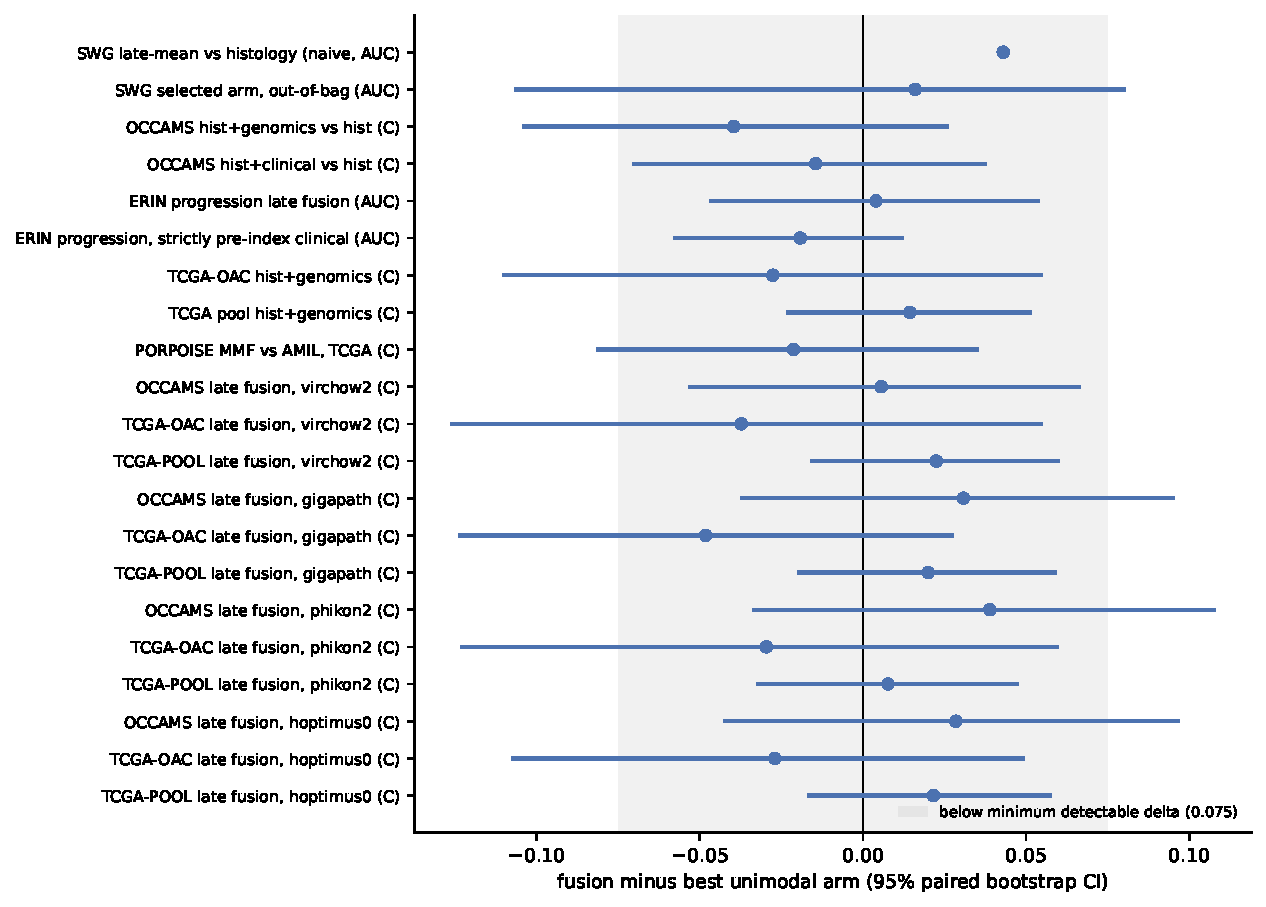
\includegraphics[width=\textwidth]{fig_fusion_forest}
\caption{Every fusion-versus-best-unimodal contrast in the thesis, as the paired-bootstrap difference in AUC or concordance. The shaded band is the smallest difference any of these cohorts can detect at 80\% power (Section~\ref{sec:power}). The first SWG row is the naive full-sample difference behind the original headline; the second is the same arm's difference when it is selected in-bag and evaluated out-of-bag.}
\label{fig:forest}
\end{figure}

\begin{table}[htbp]
\centering\small
\caption{Pre-registered confirmatory family under Holm's procedure. The SWG contrast survives Holm but not the selection adjustment of Section~\ref{sec:swg_result}, and is demoted to exploratory by the rule pre-registered for that test.}
\label{tab:holm}
\begin{tabular}{@{}llrrl@{}}
\toprule
Contrast & Metric & $p$ raw & $p$ Holm & Status \\
\midrule
SWG late-mean fusion vs histology & AUC & 0.0024 & 0.0096 & demoted (selection-adjusted $p$ = 0.25) \\
OCCAMS fusion vs histology & C & 0.231 & 0.692 & null \\
ERIN progression fusion vs histology & AUC & 0.876 & 1.0 & null \\
Keyword vs jury training labels & AUC & 0.945 & 1.0 & indistinguishable \\
\bottomrule
\end{tabular}
\end{table}

\section{Part A: is genotype visible in H\&E at all?}
\label{sec:visibility}

Fusion can only help if the second modality carries information the image does not already contain, and the converse question, whether the image already contains the genotype, was tested first. Pooled probes over 446 OAC and gastro-oesophageal cases (mean-pooled UNI2 features, PCA to 64 dimensions, logistic regression) predicted TP53 mutation at AUC 0.678 and whole-genome doubling at 0.703, against shuffled-label values of 0.50 and 0.51; stage reached 0.644 and age 0.569. An amendment of 21 August 2026 recorded this as evidence that genotype is ``partially recoverable at adequate $n$'', and a matched-$n$ learning curve was run to separate sample size from population.

\begin{figure}[htbp]
\centering
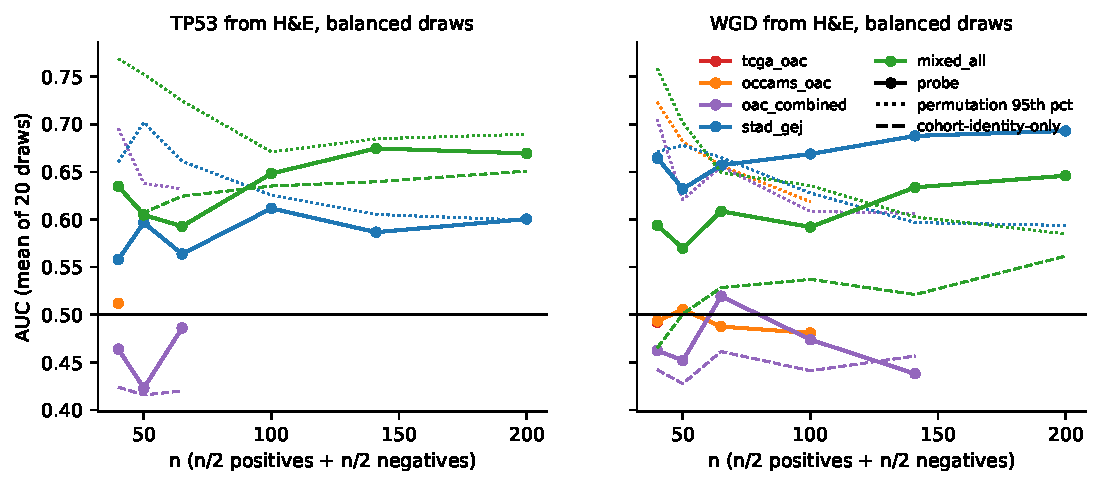
\includegraphics[width=\textwidth]{fig_visibility_matched}
\caption{Genotype visibility with class prevalence matched: every draw contains $n/2$ positives and $n/2$ negatives. Solid lines are probe AUC (20 draws), dotted lines the 95th percentile of within-cohort label permutations, dashed lines a predictor given only cohort identity. OAC strata sit at or below chance; the mixed-cohort TP53 curve is matched by cohort identity alone.}
\label{fig:visibility}
\end{figure}

The matched curve initially appeared to support a population effect: OAC at chance at every $n$, gastric/GEJ rising. An external reviewer pointed out that the curves matched total $n$ but not prevalence, and that TP53 mutation is present in about 83\% of the OAC slice and 46\% of STAD/GEJ. Re-running with balanced draws (Figure~\ref{fig:visibility}) settled the question in a way the earlier version could not. Within OAC (TCGA-OAC, OCCAMS-OAC and their union) TP53 and WGD probes score 0.42 to 0.52, below every permutation 95th percentile; the OAC strata have so few TP53-wild-type cases that balanced draws cap at $n=65$, which is stated as a limit rather than hidden. STAD/GEJ shows a modest real WGD signal, 0.63 to 0.69, clearing its permutation null from $n=100$, and marginal TP53 (0.56 to 0.61). The mixed-cohort TP53 curve at 0.63 to 0.67 is matched by a logistic model whose only input is cohort membership (0.63 to 0.65): the pooled probes were learning which cohort a slide came from. For WGD the identity-only baseline is 0.47 to 0.56 against 0.59 to 0.65, so some signal survives, consistent with the STAD result.

The conclusion of the 21 August amendment is therefore withdrawn \claim{C6b}. Genotype is not recoverable from H\&E within oesophageal adenocarcinoma at the sample sizes available, and the apparent recovery at scale was population mixture. A companion experiment on OCCAMS conditioned the attention module on genomic status and found the attention maps essentially unchanged (Spearman 0.984 between conditioned and unconditioned attention, concordance 0.576 versus 0.569), the same message from a different direction. The fusion question is therefore one of complementarity beyond what is visible, which is what the rest of the chapter tests.

\section{The SWG Barrett's cohort: a result that survived Holm and not selection}
\label{sec:swg_result}

The SWG release compares seven arm families on frozen patient folds: image-only, CNV-only, early fusion, intermediate fusion, co-attention fusion, late-mean fusion and a stacked-logit late fusion. Late-mean fusion was best on every metric (AUPRC 0.630, AUC 0.774) against image-only (AUPRC 0.557, AUC 0.731) and CNV-only (AUC 0.663). The pre-registered contrast, late-mean minus image-only AUC, gave +0.043 with a raw $p$ of 0.0024 and Holm-adjusted 0.0096, the only confirmatory test in the thesis to reject. Complementarity analyses supported it: in nested logistic models on the patient-level OOF risks, CNV risk added to histology risk (likelihood-ratio $p = 0.007$) and histology to CNV ($p = 3\times10^{-5}$).

Two things were known to qualify this. The winner's curse had been measured: late-mean won 72.8\% of 500 bootstrap re-selections, with an optimism of +0.027 AUPRC between its in-resample and full-sample scores. Against a GigaPath-encoded histology arm rather than the UNI2 one, only the Brier-score difference excluded zero ($-0.048$, [$-0.085$, $-0.011$]); AUC (+0.041, [$-0.020$, +0.103]) and AUPRC did not, so the gain was already known to be encoder-conditional. The plan filed the selection issue as ``partially known'' on this basis. An external review of the complete results (Appendix~\ref{app:review}) rated it a blocker, and the selection-adjusted test of Section~\ref{sec:selection_method} was pre-registered with a decision rule: the claim stands if the adjusted $p$ is below 0.05 \emph{and} the out-of-bag delta's interval excludes zero; otherwise it is demoted to exploratory.

\begin{figure}[htbp]
\centering
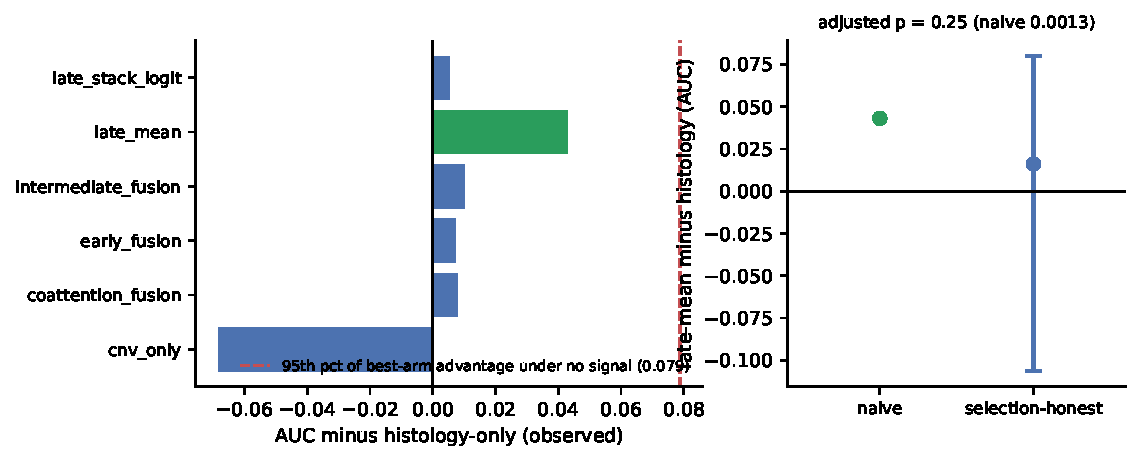
\includegraphics[width=\textwidth]{fig_selection_adjusted}
\caption{Selection-adjusted inference for the SWG headline. Left: each arm's observed AUC advantage over image-only; the dashed line is the 95th percentile of the \emph{best} arm's advantage under 20,000 patient-level label permutations. Right: the late-mean gain as reported (naive) and as obtained when the arm is selected in-bag and evaluated out-of-bag (2,000 resamples).}
\label{fig:selection}
\end{figure}

Both criteria failed (Figure~\ref{fig:selection}). The 95th percentile of the best fusion arm's advantage under no signal is 0.079, almost twice the observed 0.043; the adjusted $p$ is 0.253 over the five fusion arms and 0.368 if CNV-only is allowed into the candidate set, against an unadjusted single-arm permutation $p$ of 0.0013. The selection-honest delta is +0.016 with interval [$-0.106$, +0.080]; late-mean is selected in 69\% of resamples and its out-of-bag delta is positive in 72\% of them. The gap between the naive 0.043 and the honest 0.016 is 0.027, the same optimism the winner's-curse analysis had estimated independently. AUPRC was marginal (adjusted $p$ 0.040 for fusion arms only, 0.099 for all arms) and was not the pre-registered metric. Claim C1 is demoted \claim{C1}: the thesis reports SWG fusion as a positive but selection-unadjusted advantage of uncertain size, and the honest estimate of the effect a user would obtain after selecting is +0.016 AUC.

Two further SWG analyses belong here. The GigaPath contrast's Brier result is reported as a Brier improvement, not as evidence of better calibration, since the Brier score mixes calibration with discrimination and no reliability analysis was run. And the SWG cohort's 36\% patient overlap with ERIN (Section~\ref{sec:independence}) does not affect any within-SWG result, because no SWG model was trained on ERIN.

\section{OCCAMS: fusion trends harmful}
\label{sec:occams_result}

On 87 OCCAMS resection cases with 58 deaths, the histology arm reaches concordance 0.627 [0.539, 0.711]; WGS-derived genomics (TP53 flags, ploidy, WGD) 0.521 [0.434, 0.602]; seven clinical fields 0.536 [0.458, 0.624]. Late fusion of histology with genomics gives 0.589, a difference of $-0.040$ [$-0.104$, +0.026] against histology; with clinical, 0.613 ($-0.015$ [$-0.070$, +0.038]). The pre-registered contrast has Holm $p$ 0.69 \claim{C2}.

A reviewer asked whether pooling five folds' Cox risks understated the concordance. It does, slightly: fold-specific risk offsets range from $-1.12$ to $-0.15$, and the within-fold concordance of histology is 0.655 against the pooled 0.627 (Section~\ref{sec:withinfold}). Re-computing late fusion with fold-local z-scoring gives hist+genomics 0.600 ($-0.029$ [$-0.095$, +0.036] against histology) and hist+clinical 0.629 (+0.002 [$-0.059$, +0.062]). Per-fold concordance spans 0.54 to 0.79, the instability the power map predicts at $n=87$. Fifty-permutation controls place the shuffled-label concordance of 0.574 from an early run inside the legitimate null spread.

\section{ERIN: the clinical arm's signal was leakage}
\label{sec:erin_result}

ERIN slide-level progression (153 index slides, 28 progressors) is predicted from histology at AUC 0.819 [0.723, 0.900]. The clinical arm built from report-derived fields scores 0.564; late fusion 0.823 (+0.004 [$-0.047$, +0.054]). An ablation restricting clinical fields to those strictly available before the index date drops the clinical arm to 0.480 and fusion to 0.800 ($-0.019$ [$-0.058$, +0.012]): what signal the clinical arm had came from fields that encode the index date itself. The pre-registered contrast has Holm $p$ 1.0 \claim{C3}. The permutation control for the histology arm (75 permutations) gives a null mean of 0.502 and empirical $p$ of 0.013.

\begin{figure}[htbp]
\centering
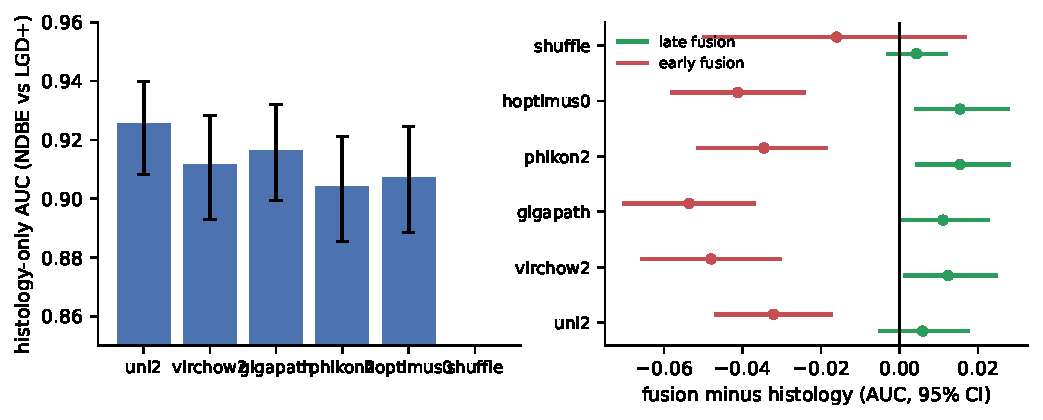
\includegraphics[width=\textwidth]{fig_erin_encoders}
\caption{ERIN dysplasia grade (NDBE vs LGD+, 2,153 slides) across five tile encoders. Left: histology-only AUC. Right: late and early fusion of report-derived clinical fields with histology, as paired differences against histology.}
\label{fig:erin_encoders}
\end{figure}

On the easier grade endpoint (Figure~\ref{fig:erin_encoders}) histology alone is near ceiling: 0.926 [0.908, 0.940] with UNI2, 0.912 to 0.916 with the other encoders. Late fusion with clinical fields adds +0.006 [$-0.005$, +0.018] on UNI2 and +0.011 to +0.015 with intervals excluding zero on four of the other encoders; early fusion hurts on every encoder ($-0.032$ to $-0.054$). The late-fusion gains are real but an order of magnitude below the minimum detectable delta for any of the survival cohorts, and they sit on top of a 0.93 baseline; they are reported as exploratory.

\section{TCGA}
\label{sec:tcga_result}

TCGA-OAC (65 cases, 36 deaths): histology 0.679 [0.567, 0.776], genomics 0.537, clinical 0.597; hist+genomics 0.651 ($-0.028$ [$-0.110$, +0.055]); hist+clinical 0.688. The gastro-oesophageal pool (399, 176 deaths): histology 0.547 [0.501, 0.595], genomics 0.540, clinical 0.623; hist+genomics 0.562 (+0.014 [$-0.023$, +0.051]). Hist+clinical in the pool is the one contrast in the thesis whose interval excludes zero in fusion's favour (+0.061 [+0.027, +0.095]), and it is not a genomics result: the clinical arm alone (0.623) beats histology (0.547) in this pool because stage is in the clinical table. The OAC subgroup's histology concordance within the pooled model is 0.682, close to the OAC-only model, so pooling neither helps nor harms the OAC cases. The pooled histology concordance is low because STAD and OAC survival differ and a single histology model is being asked to rank across them.

\section{Encoder sweep and a published architecture}
\label{sec:porpoise}

The encoder escape hatch (``fusion would have worked with a better image representation'') was closed by repeating the three survival fusion analyses with Virchow2, GigaPath, Phikon-v2 and H-Optimus-0 features. All twelve late-fusion contrasts have intervals spanning zero (Figure~\ref{fig:forest}, lower rows) \claim{C4}. Histology-only concordance varies with encoder (OCCAMS 0.49 to 0.63), consistent with published reports that no encoder dominates across tasks, and no encoder makes fusion win.

The architecture escape hatch was closed with PORPOISE \citep{chen2022porpoise}, run from its published classes and loss on 439 TCGA slides with the published gene-signature molecular input (8,827 features) and frozen splits, with only the first linear layer widened from 1,024 to 1,536 to accept UNI2 features. Its multimodal model (MMF) reached concordance 0.545 against its own attention-MIL unimodal baseline at 0.566, a difference of $-0.021$ [$-0.081$, +0.035] \claim{C5}. The interval permits a gain of up to +0.035; what it rules out is the gain of roughly 0.05 to 0.10 that the published pan-cancer results would predict.

\section{The power map}
\label{sec:power}

\begin{figure}[htbp]
\centering
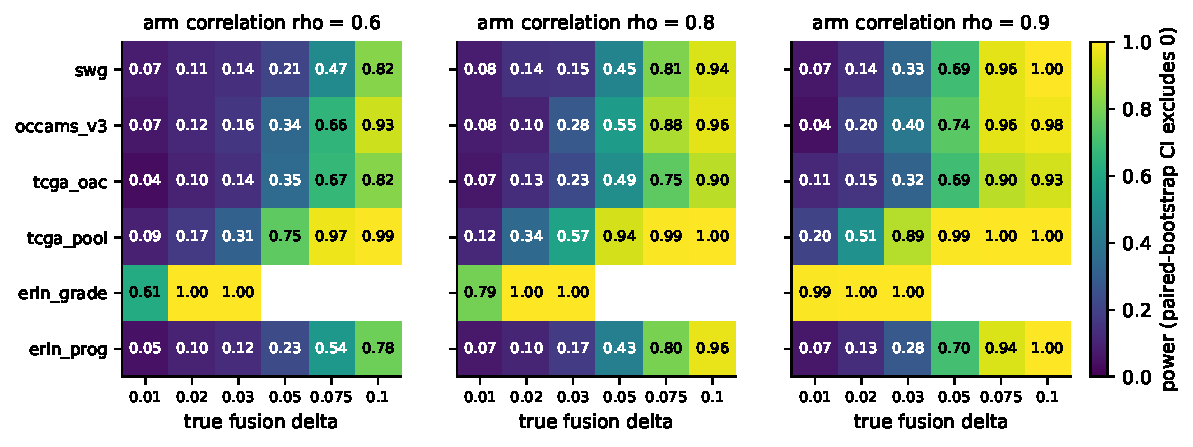
\includegraphics[width=\textwidth]{fig_power_map}
\caption{Simulated power to detect a true fusion gain (paired-bootstrap interval excluding zero) as a function of the gain and the correlation between the two arms' scores, for each cohort's $n$, events and observed baseline. ``n/a'' marks gains that would push the true metric above 0.99.}
\label{fig:power}
\end{figure}

Figure~\ref{fig:power} is the thesis's explanation of its own nulls. At an arm correlation of 0.8, the smallest gain detectable at 80\% power is 0.075 in SWG, OCCAMS and ERIN progression, 0.10 in TCGA-OAC and 0.05 in the 399-case TCGA pool; at the Holm worst-case threshold these step up to 0.10. The observed fusion differences (Figure~\ref{fig:forest}) run from $-0.04$ to +0.04. Type-I error at zero effect is 1.0 to 4.5\% across cells (nominal 2.5\% one-sided, Wilson half-width about 3\% at 200 replicates), so the detection rule is not anti-conservative. An earlier version of this map paired the ERIN grade cohort's patient count with a slide-level baseline and silently clipped gains that exceeded 1.0; both were fixed after review and neither changed the fusion-cohort numbers by more than one grid step \claim{C6}.

The map licenses one sentence and forbids another. It licenses: ``no available oesophageal cohort can detect a fusion gain below 0.075; the observed gains are smaller than that.'' It forbids: ``fusion does not help.'' The thesis uses the first.

\section{Cross-cohort transfer}
\label{sec:transfer}

\begin{figure}[htbp]
\centering
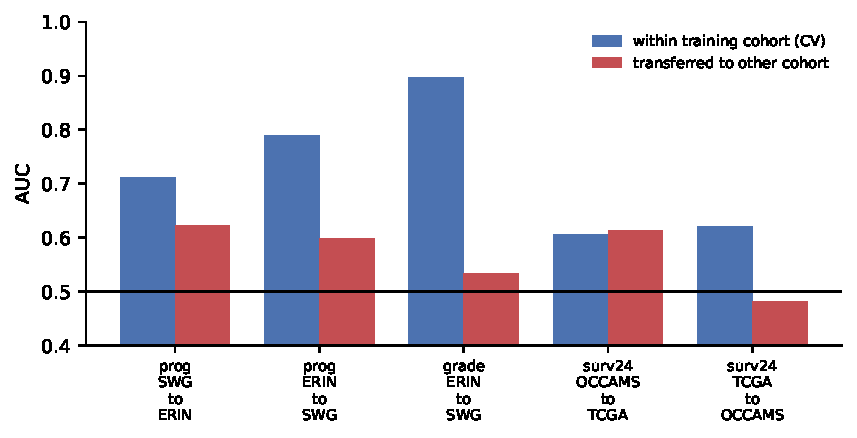
\includegraphics[width=0.85\textwidth]{fig_transfer_matrix}
\caption{Pooled-feature probes trained in one cohort and evaluated in another, with the 54 SWG patients shared with ERIN removed. Within-cohort cross-validated AUC is shown for comparison.}
\label{fig:transfer}
\end{figure}

A pooled-feature probe (mean UNI2, PCA, logistic) trained in one cohort and applied to another loses most of its performance (Figure~\ref{fig:transfer}). After removing the 54 overlapping patients, SWG-to-ERIN progression transfers at 0.62 (within-cohort 0.71), ERIN-to-SWG at 0.60 (within 0.79), ERIN grade to SWG pathologist grade at 0.53 (within 0.90); OCCAMS-to-TCGA 24-month survival at 0.61 and TCGA-to-OCCAMS at 0.48. Removing the overlap moved the three Barrett's cells by at most 0.05 and did not change the conclusion; the pre-overlap numbers (0.64, 0.54, 0.56) are superseded.

\section{Distilling a molecular teacher}
\label{sec:wgd}

An attention-MIL teacher trained on 562 resection cases with WGS labels predicts WGD at AUC 0.730 [0.689, 0.773] and TP53 mutation at 0.764 [0.722, 0.803] in-domain. Applied to ERIN surveillance biopsies, the predicted-WGD score is \emph{inversely} associated with progression (AUC 0.315; mean score 0.36 in progressors, 0.56 in non-progressors), and in SWG it correlates weakly negatively with measured copy-number complexity (Spearman $-0.10$, $p=0.005$). Neither cohort measures WGD directly, so these are stated as they are: an inverse association with progression and a weak negative association with CNV complexity, not a demonstration that the teacher mis-ranks true WGD \claim{C9}. The plausible reading is a specimen-type shift between resections and biopsies, and the practical one is that a resection-validated ``virtual biomarker'' should not be assumed to carry over to surveillance material.

\section{Longitudinal trajectories}
\label{sec:trajectory}

Two cohorts allow a trajectory model. In ERIN (153 patients, 32 with more than one time point) hand-built trajectory features underperform the index slide alone (0.710 versus 0.780, $-0.070$ [$-0.123$, $-0.018$]) and a GRU over the sequence matches it (+0.010 [$-0.054$, +0.073]). In SWG, with about 4.7 samples per patient, no trajectory arm beat the last-sample snapshot on the frozen folds (\resfile{results/swg\_trajectory.json}). A secondary observation that current H\&E predicts the next biopsy's copy-number complexity (Spearman 0.161, $p=1.3\times10^{-4}$) prompted a follow-up with baselines it had lacked.

\begin{figure}[htbp]
\centering
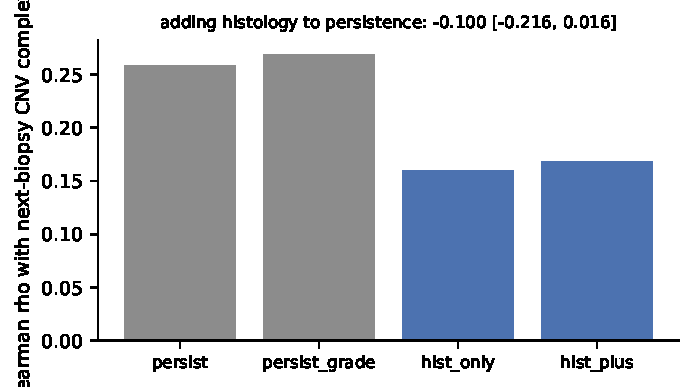
\includegraphics[width=0.7\textwidth]{fig_trajectory_baselines}
\caption{Predicting the next biopsy's CNV complexity in SWG (557 transitions, 124 patients). Persistence of the current CNV state, with elapsed time and current grade, outperforms histology, and adding histology to persistence does not help.}
\label{fig:trajectory}
\end{figure}

Current CNV complexity and elapsed time alone predict the next value at Spearman 0.259 (0.269 with the current grade added); histology alone 0.160; histology added to the persistence baseline 0.168 (Figure~\ref{fig:trajectory}). The increment from histology is $-0.100$ with a patient-clustered interval of [$-0.216$, +0.016]. The reading ``images anticipate genomic evolution'' is withdrawn \claim{C10}; histology was recovering part of the current CNV state, which the current CNV measurement recovers better.

\section{What this chapter licenses}

Seven fusion families, four encoders, a published architecture and four cohorts produced no fusion gain whose interval excludes zero after selection is priced in, and the one that appeared to was explained by selection. Three mechanisms that would have produced a false positive in a conventional analysis were caught: selecting the best arm on the evaluation data, sharing patients across cohorts, and pooling populations with different prevalence. The power map says the true gain, if any, is below what these cohorts can see. Chapter~\ref{ch:discussion} turns these into a protocol.

\chapter{Report-derived supervision and how to validate it}
\label{ch:labels}

Histology models reach clinical-grade performance at tens of thousands of slides \citep{campanella2019}, and no pathologist will re-grade tens of thousands of slides for a research project. The labels have to come from the reports that already exist. This chapter builds three ways of extracting them, validates them against each other and against human registry grades, and then measures something the report-derived-label literature has not measured: how wrong the standard shortcut of assigning a report's worst grade to every slide of the case actually is, and whether it matters.

\section{Three label sources}

\paragraph{Keyword ladder.} \texttt{pathladder} is a deterministic extractor: sentence splitting, windowed negation, and worst-finding-wins over the ordinal ladder NDBE $<$ IND $<$ LGD $<$ HGD $<$ CANCER; a second schema covers TCGA resection reports. On 507 TCGA ESCA and STAD reports it recovers histologic type with 98\% coverage and 100\% accuracy against GDC coding, and grade with 77\% coverage and 96.5\% accuracy against the cBioPortal clinical record.

\paragraph{Feasibility grader.} An earlier, single-model labelling from the project's feasibility phase, retained as a third source because it is known to be noisy and therefore useful for asking whether label noise propagates.

\paragraph{Language-model jury.} Eight open-weight models (Section~\ref{sec:jury_method}) each grade every report; a label is accepted when a clear majority agree, near-splits become \emph{unsure}, and the hardest 78 disagreements were adjudicated by a reviewer reading the full text on the cluster. Over 7,149 reports the jury produced 6,867 train-eligible labels (NDBE 5,151, CANCER 863, HGD 405, LGD 269, IND 257), 204 unsure and 78 adjudicated (Figure~\ref{fig:jury}). Parse rates were 100\% for every model except llama3.1-8B at 98.3\%.

\begin{figure}[htbp]
\centering
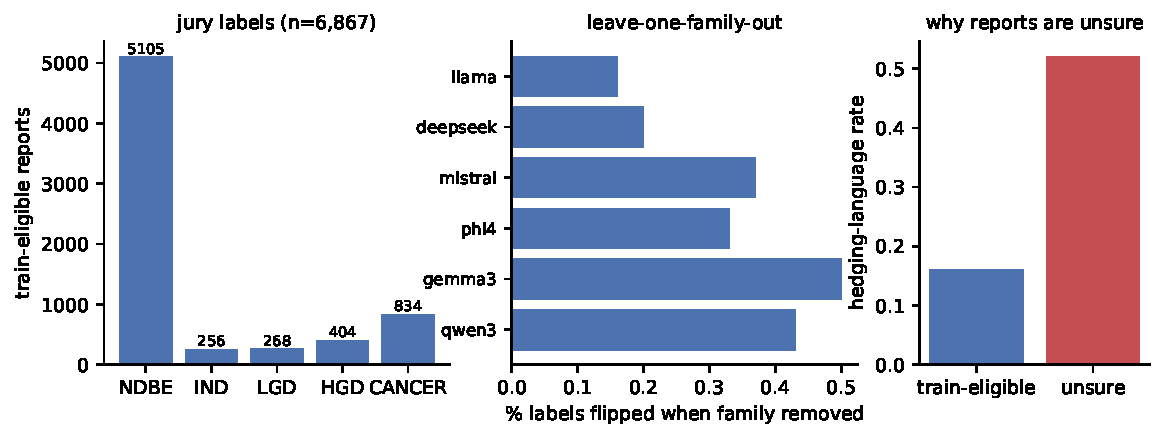
\includegraphics[width=\textwidth]{fig_jury}
\caption{The ERIN jury. Left: label distribution of the 6,867 train-eligible reports. Middle: fraction of labels that change when one model family is removed from the jury. Right: rate of hedging language in reports the jury labels confidently versus those it holds out as unsure.}
\label{fig:jury}
\end{figure}

\section{Is the jury robust, and does its uncertainty mean anything?}

Removing any one model family and re-voting flips at most 0.5\% of labels (gemma3 is the most load-bearing family) and changes the eligible set with Jaccard at least 0.979 \claim{C12}. The unsure reports are not random: they carry hedging language at 3.3 times the rate of confident reports (0.52 versus 0.16 per report) and more addenda \claim{C13}. A grade model trained on the eligible slides scores 0.926 on them and only 0.697 against the jury's plurality on the 59 unsure slides, while its own confidence fails to flag them (62.7\% ``confident'' predictions on unsure slides versus 73.2\% on eligible). Deferring the model's least confident 5, 10 and 20\% of slides raises AUC from 0.926 to 0.931, 0.936 and 0.945. Holding the unsure reports out of training is therefore justified twice over: they are ambiguous in the text, and the image model cannot tell.

\section{Do label sources matter downstream?}
\label{sec:labelsource}

\begin{figure}[htbp]
\centering
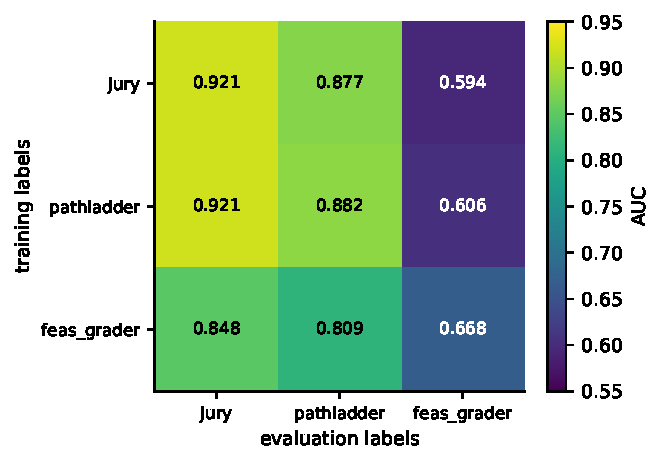
\includegraphics[width=0.55\textwidth]{fig_labelsource_xeval}
\caption{Grade models trained on each label source, evaluated against each label source (AUC, 2,153 ERIN slides). Jury- and keyword-trained models are interchangeable; the noisy feasibility grader is not.}
\label{fig:xeval}
\end{figure}

Models trained on jury labels and on keyword-ladder labels are indistinguishable when both are evaluated against jury labels (0.921 versus 0.921, difference +0.0003 [$-0.008$, +0.009]; Holm $p$ 0.945, the fourth confirmatory contrast) \claim{C16}, and against keyword labels (0.877 versus 0.882). The feasibility grader's model trails by 0.073 [$-0.094$, $-0.053$] and no model predicts the feasibility grader's own labels well (0.59 to 0.67), which locates the noise in that labeller rather than in the images (Figure~\ref{fig:xeval}). The practical reading is that a validated keyword extractor is sufficient supervision for coarse grade, and that a jury earns its cost on the harder tasks below. Where the two disagree on ERIN (agreement 81.7\% on 6,867 reports), the dominant confusion is the ladder calling CANCER where the jury says NDBE (321 cases), almost all in reports that mention cancer in a negated or historical context.

\section{External validation against human grades}
\label{sec:pancancer}

The jury had never seen a TCGA report or a non-Barrett's cancer. The same pipeline, with the five jurors available at the time and a G1--G4/high/low schema, graded 1,294 TCGA reports in four cancer types with registry grades from cBioPortal.

\begin{figure}[htbp]
\centering
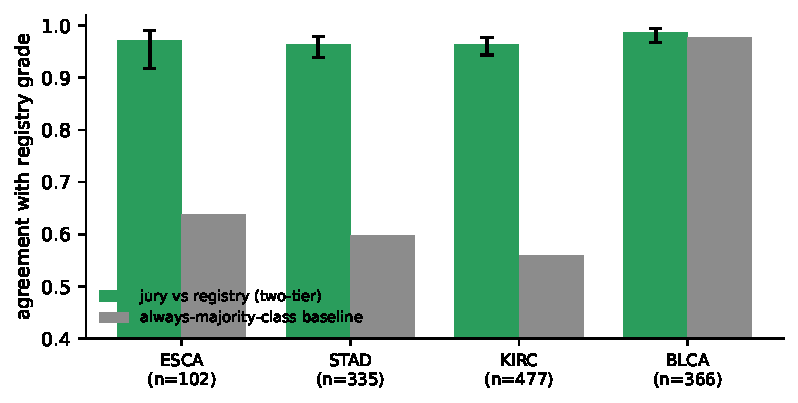
\includegraphics[width=0.8\textwidth]{fig_pancancer}
\caption{Agreement between jury grade and the human registry grade (two-tier low/high), with Wilson 95\% intervals, against the agreement an always-majority-class labeller would achieve.}
\label{fig:pancancer}
\end{figure}

Two-tier agreement is 0.971 in ESCA ($n=102$), 0.964 in STAD (335) and 0.964 in KIRC (477), against always-majority-class baselines of 0.637, 0.597 and 0.560; balanced accuracy is 0.963 to 0.967, macro-F1 0.963 to 0.968 and minority-class recall 0.946 to 0.991 (Figure~\ref{fig:pancancer}) \claim{C14}. BLCA's exact agreement of 0.579 puzzled an early draft; the registry codes only high/low (358/8) while the jury emitted G2, G3, G4 and high, so the mismatch was a coding scheme, and after mapping all 8 low-grade cases are recovered. Its two-tier figure of 0.986 is barely above the 0.978 majority baseline and is reported as uninformative beyond minority recall. Replaying the five-juror rule on the saved ERIN votes agrees with the deployed eight-juror rule on 99.4\% of 6,657 common reports (eligibility Jaccard 0.991), so the TCGA procedure is a faithful proxy for the ERIN one.

\section{Deliberation versus voting}

Published frameworks run language models as a multidisciplinary team meeting rather than a vote \citep{mdteamgpt2025, nussinov2024mdt}. On the 280 hardest ERIN cases (adjudicated plus unsure), three consultant models gave independent first-round opinions with quoted evidence, saw each other's opinions and could rebut, and a chair model issued a verdict. On the 78 adjudicated cases the chair was right on 77 (98.7\%) against 76 for the first-round majority (97.4\%), with no case in which deliberation talked a correct majority out of the right answer; 85 of 124 first-round disagreements converged to unanimity (Figure~\ref{fig:mdt}). That is one additional correct decision on a development benchmark, not a demonstration of superiority. On the 201 unsure cases the chair claimed confidence at or above 0.7 on 200, which is not credible for reports the jury found ambiguous; chair confidence is treated as uncalibrated \claim{C15}.

\begin{figure}[htbp]
\centering
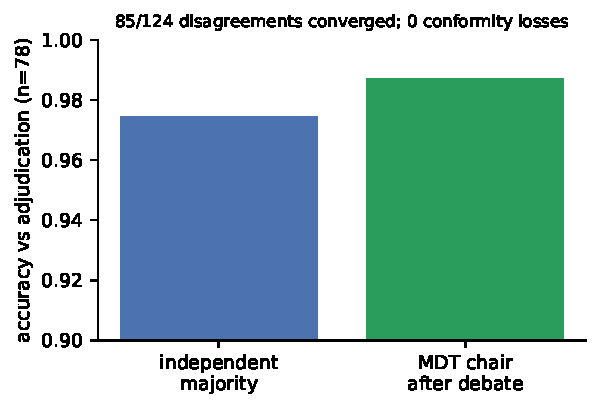
\includegraphics[width=0.5\textwidth]{fig_mdt}
\caption{Multidisciplinary-team-style deliberation against independent majority vote on the 78 adjudicated ERIN cases.}
\label{fig:mdt}
\end{figure}

\section{Sections, slides and the case-max shortcut}
\label{sec:sections}

A Barrett's surveillance report grades several biopsy sites, one lettered section each, and the sections often disagree. The report-level label of the previous sections assigns the worst grade in the report (``case-max'') to every slide from that case, which is the shortcut used in almost all report-supervised pathology work. To measure what it costs, the jury was re-run per section with a schema that returns a set of grades and cancer subtypes (adenocarcinoma, squamous, signet-ring, post-neoadjuvant treatment effect) for each lettered section. Parse failure was 0.3\%; reports averaged 2.36 sections; 18,691 section-level consensus rows were obtained over 7,031 reports, a section counting only if seen by a majority of jurors and a grade only if at least three of five listed it. Shiv Sakthivel's section-to-slide table then linked 1,538 feature slides to their own section.

\begin{figure}[htbp]
\centering
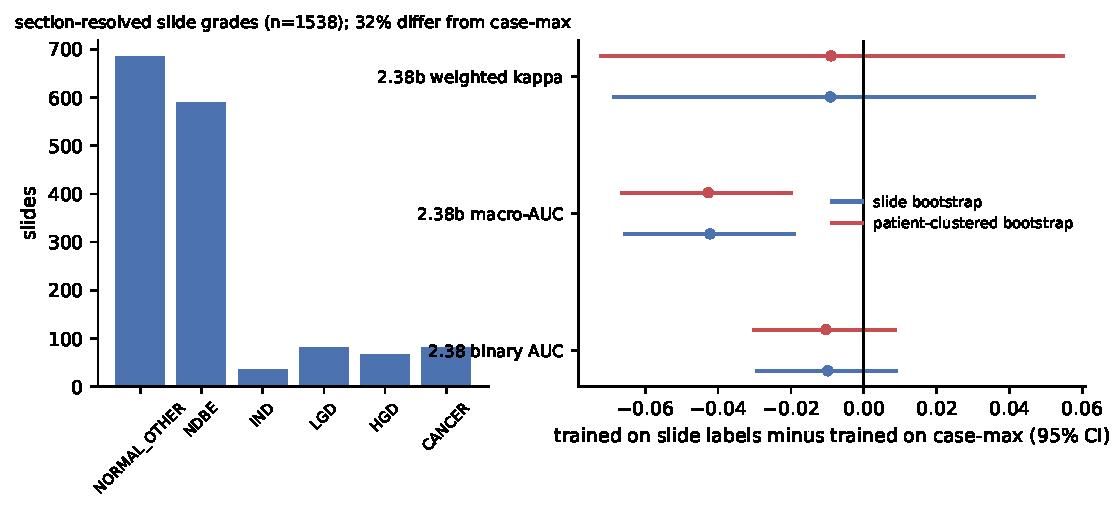
\includegraphics[width=\textwidth]{fig_slide_vs_casemax}
\caption{Left: section-resolved slide grades for the 1,538 dual-labelled slides. Right: models trained on section-resolved labels minus models trained on case-max labels, evaluated on section-resolved truth, with slide-resampled and patient-clustered bootstrap intervals.}
\label{fig:svc}
\end{figure}

\textbf{32.0\% of slides carry a different grade from their case-max label} (Figure~\ref{fig:svc}, left) \claim{C17}. Most of the difference is benign tissue in a case that contained dysplasia elsewhere: 685 of the 1,538 slides are graded normal-or-other tissue by their own section and 589 NDBE, against 82 LGD, 66 HGD, 81 cancer and 35 IND.

Whether that noise matters was tested with identical gated-attention models on identical patient-disjoint folds, trained once on case-max labels and once on section-resolved labels, and evaluated against section-resolved truth. For binary screening (LGD or worse) the answer is no: case-max-trained 0.871 [0.841, 0.898], section-trained 0.860 [0.829, 0.891], difference $-0.010$ [$-0.028$, +0.009] \claim{C18}. The natural follow-up asked whether the noise bites where it lives, at six-class grading (normal $<$ NDBE $<$ IND $<$ LGD $<$ HGD $<$ cancer), and the prediction was that section labels would win there. They lost: case-max-trained macro one-vs-rest AUC 0.764 against 0.722, difference $-0.042$ [$-0.066$, $-0.019$], quadratic-weighted kappa 0.524 against 0.515 (difference $-0.009$ [$-0.066$, +0.047]) \claim{C19}. Patient-clustered intervals (1,155 patients) are 1.00 to 1.10 times as wide and change nothing (Figure~\ref{fig:svc}, right).

The reading is a trade between label noise and sample size. With 35 IND, 66 HGD and 82 LGD slides, section-resolved labels starve the rare classes; case-max propagates the report's worst grade to every slide of the case, which is wrong for a third of slides individually but supplies several times more positive examples per rare class. At this cohort size the noisy-but-plentiful labels win. This could invert in a cohort with hundreds of slides per rare class, and the thesis states that as a testable prediction rather than a universal claim. For anyone training on report labels today, the result is reassuring: the shortcut everyone uses is safe for screening and not worse for grading at the scale most groups have.

\section{A human comparison arm}

Because the report text cannot leave the hospital network, a cluster-internal grading application was built (a standard-library HTTP server over SQLite, per-section grade and subtype check-boxes mirroring the jury schema) so that four or five laboratory members can each grade a common core of 20 reports plus 20 unique ones, giving inter-rater agreement and coverage. It is live; grading had not begun when this draft was frozen, and a pathologist arm remains the thesis's main unmet validation (Section~\ref{sec:limitations}).

\section{Barrett's natural history from labelled reports}
\label{sec:natural_history}

\begin{figure}[htbp]
\centering
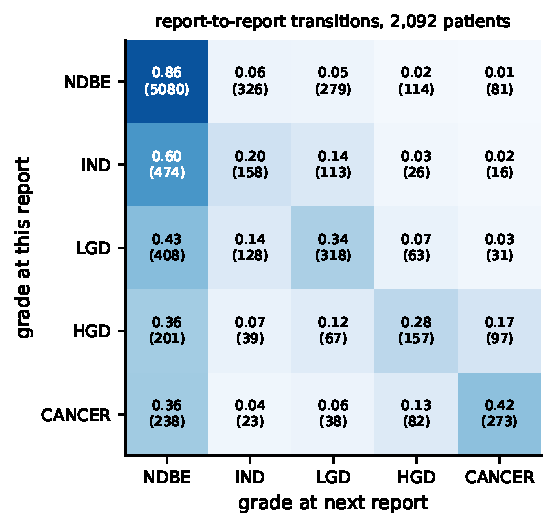
\includegraphics[width=0.6\textwidth]{fig_natural_history}
\caption{Grade-to-grade transitions between consecutive reports of the same patient, from jury-labelled reports in the Barrett's database export (row-normalised; counts in parentheses).}
\label{fig:nathist}
\end{figure}

Labelling the 13,645-report database export with the same jury (12,780 labelled, 12,255 confidently) gives grade sequences for 2,092 patients (Figure~\ref{fig:nathist}). Most NDBE reports are followed by NDBE (5,080 of 5,880 transitions); the median time from NDBE to a first dysplastic report is 1.06 years; and transitions from cancer back to NDBE (238) record post-treatment surveillance rather than regression. A text-only progression model on 8,830 reports reaches AUC 0.696. Structured-truth validation of these sequences is blocked on the database's grade-code map and is listed as pending.

\chapter{Vision-language alignment and discovery from reports}
\label{ch:vlm}

The report-slide pairs of Chapter~\ref{ch:labels} allow a second use beyond labelling: training an image model to agree with the report's text directly, so that grading needs no labels at all. This chapter reports that model and where it does and does not transfer, and closes with two uses of the labelling machinery for case-finding and phenotype discovery.

\section{A contrastive slide-report model}

Report text was embedded with a local sentence encoder (\texttt{nomic-embed-text}, 768-dimensional) and slides with a gated-attention tower over UNI2 tiles (512 to 768 dimensions); the two were trained CLIP-style \citep{radford2021clip} to place each slide near its own report. A signal test on 2,153 pairs with a linear text projection gave slide-to-report recall@1 of 0.037 against a chance of 0.0023 (16 times chance) and zero-shot grading, by comparing each slide to two prompt embeddings (``negative for dysplasia'' versus ``dysplasia or worse''), at AUC 0.823 against a supervised reference of 0.90. Full training on a patient-disjoint split (1,333 train, 452 validation, 436 test slides) reached recall@1 of 0.028 (12 times chance) and recall@5 of 0.123 on the ERIN test fold, and zero-shot grade AUC 0.889 \claim{C22}. The supervised model on the same task scores 0.926; the vision-language model gets to 0.889 with no labels.

\begin{figure}[htbp]
\centering
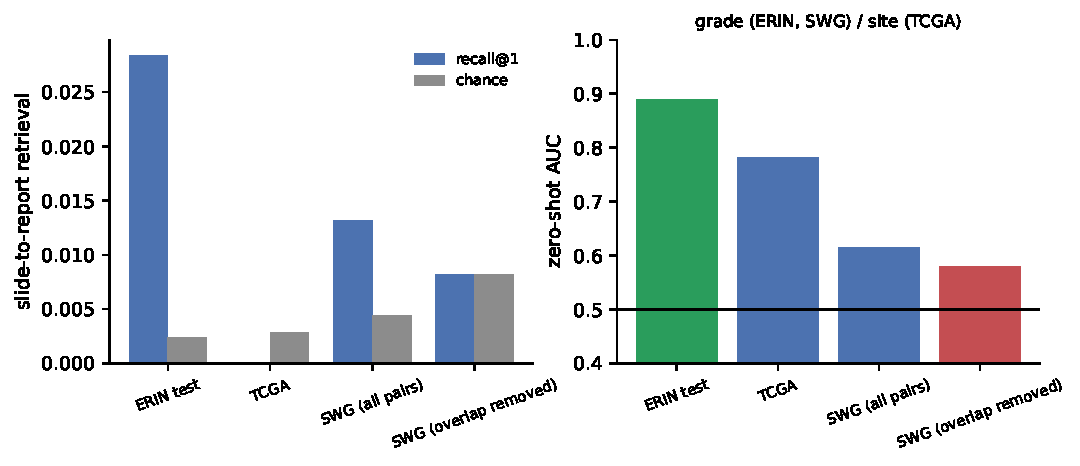
\includegraphics[width=\textwidth]{fig_vlm}
\caption{The slide-report model within ERIN and on two external cohorts. Left: slide-to-report retrieval against chance. Right: zero-shot AUC for grade (ERIN, SWG) or tissue site (TCGA). The SWG result is shown before and after removing the 54 SWG patients who are also ERIN patients.}
\label{fig:vlm}
\end{figure}

\section{Transfer}

On 350 TCGA slide-report pairs, retrieval collapses (recall@1 of 0.0, recall@5 of 0.017) while a zero-shot site classification (oesophagus versus stomach) still reaches 0.782: the semantics carry, the literal report style does not \claim{C23}. SWG initially looked like a partial success: on 227 SWG slides matched to Barrett's-database reports by accession number, retrieval was three times chance and zero-shot grading against the pathologist's grade scored 0.614. The overlap audit (Section~\ref{sec:independence}) then showed that 105 of those 227 pairs came from the 54 patients shared with ERIN, exactly the patients most likely to have a matching database report. On the 122 clean pairs, recall@1 is 0.0082, which is $1/122$, and zero-shot AUC is 0.579 on 9 positives (Figure~\ref{fig:vlm}). The SWG half of the claim is demoted: the ERIN-trained model shows no demonstrated transfer to either external cohort. Within ERIN it remains a label-free grader at 0.889.

A separate test asked whether disagreement among five foundation-model encoders on the same slide carries information: it does not correlate with jury entropy (Spearman 0.042), does not flag unsure reports (AUC 0.52) and does not predict progression (0.52). Encoder disagreement is not a usable uncertainty signal here.

\section{Case-finding: eosinophilic oesophagitis}

Eosinophilic oesophagitis is coded inconsistently and hides in surveillance corpora. A keyword screen followed by a five-model jury with a four-way schema (diagnosed, suspected, negated or incidental, absent) and eosinophil-count extraction classified 26 reports from 17 patients as diagnosed (13 unanimously) and 77 reports from 66 patients as suspected, with the remaining 688 keyword-positive reports negated or incidental; none of 100 keyword-negative control reports was classified as either \claim{C24}. These are language-model classifications, not verified diagnoses, and the 0 of 100 is on sampled keyword-negative controls whose true status was not independently established; the output is a candidate list for a clinician, delivered in a day from 7,149 reports.

\section{Open-vocabulary phenotypes}

A pilot asked the jury to list every histological finding in a report without a fixed schema. Over 1,000 reports it returned 844 distinct terms; the fifty most frequent are the expected surveillance vocabulary (intestinal metaplasia 646, Barrett's oesophagus 611, chronic inflammation 581, squamous mucosa 253, high-grade dysplasia 129, low-grade dysplasia 106, adenocarcinoma 73) with a long tail (p53 over-expression 34, lymphovascular space invasion 30, fundic gland polyp 42) \claim{C25}. The pilot establishes feasibility for a full-corpus phenotype atlas, which is planned as a separate paper and was not run for this thesis.

\chapter{Discussion}
\label{ch:discussion}

\section{What was found}

The thesis set out to add a second modality to H\&E in oesophageal cancer and ended up documenting, in some detail, why the field's positive results in this area should be read cautiously. Four cohorts, seven fusion families, five encoders and a published architecture produced no fusion gain that survives three checks: selection-adjusted inference, a patient-overlap audit and prevalence-matched comparison. Each check removed a result that had looked real. Selection removed the SWG headline, which had passed a pre-registered Holm-corrected test and had a measured winner's curse filed as ``small''; the honest effect is +0.016 AUC with an interval from $-0.11$ to +0.08. The overlap audit removed the vision-language model's SWG transfer, which was carried by the third of SWG patients who are also ERIN patients. Prevalence matching removed the finding that genotype is visible in H\&E at pooled scale, which a cohort-identity predictor reproduced. A power map explains the rest: the cohorts that exist for this disease cannot see gains below 0.075, and the observed gains are smaller.

On the supervision side the findings are positive and specific. A jury of eight local language models labels surveillance reports in a way that does not depend on any one model, whose uncertainty tracks hedged text, and that agrees with human registry grades at 0.96 to 0.97 in three cancer types it never saw. A deterministic keyword ladder trains models as good as the jury does for coarse grade. Re-labelling at the section level showed the standard case-max shortcut mislabels 32\% of slides, and then showed the shortcut is no worse for screening and better for six-class grading at this cohort size, because the extra positives it propagates outweigh the noise. A contrastive slide-report model grades held-out ERIN slides at 0.889 with no labels and does not transfer.

\section{A protocol for claiming a fusion gain}
\label{sec:protocol}

Every rule below is motivated by a specific failure in this thesis. Appendix~\ref{app:p2} develops them as a paper.

\begin{enumerate}
\item \textbf{Adjust for arm selection before reporting the best fusion arm.} Report the max-over-arms permutation $p$ and the out-of-bag delta of the selected arm. The SWG result went from $p=0.0096$ to $p=0.25$ (Section~\ref{sec:swg_result}).
\item \textbf{Audit patient overlap across every pair of cohorts treated as independent}, using identifiers that actually travel between them (here, accession numbers), not anonymised study IDs. A ``6 of 1,992'' overlap was 54 of 150 (Section~\ref{sec:independence}).
\item \textbf{Match prevalence when comparing populations or pooling cohorts}, and always fit a cohort-identity-only baseline for any pooled model (Section~\ref{sec:visibility}).
\item \textbf{Report the minimum detectable gain for your cohort before interpreting a null}, and refuse to write ``fusion does not help'' when the interval merely fails to exclude zero (Section~\ref{sec:power}).
\item \textbf{Use patient-clustered bootstraps, within-fold concordance and fold-local normalisation for late fusion.} In this thesis these changed no conclusion, which is the reason to run them: they cost minutes and remove a class of objection (Sections~\ref{sec:clustered}, \ref{sec:withinfold}).
\item \textbf{Pre-register the confirmatory family and record every promotion and demotion with a date.} Three conclusions in this thesis changed after pre-registered decision rules were applied to new tests; the rules were written before the results existed, so none of the changes could be argued away (Appendix~\ref{app:plan}).
\end{enumerate}

The protocol does not say fusion fails. It says what a fusion claim has to survive, and it notes that several claims in the literature have not been asked to.

\section{Limitations}
\label{sec:limitations}

\begin{itemize}
\item No pathologist re-graded slides. All ERIN labels are report-derived; the external anchors are TCGA registry grades and 78 human-adjudicated reports. A grading application is live and a pathologist arm is the first item of future work.
\item Rare-class counts are small (35 IND, 66 HGD, 82 LGD slides), so the six-class result of Section~\ref{sec:sections} is a statement about this cohort size, with the reversal at larger $n$ stated as a prediction.
\item Jury labels and section labels share provenance, and the models that evaluate them are trained on them; the circularity is broken only where external anchors exist.
\item ERIN is a single site; SWG is 150 patients; OCCAMS attrition to 87 is data-availability, not selection, but it is still 87.
\item The chair's confidence in the deliberation experiment is uncalibrated; the vision-language model is trained and validated on one site; the WGD-teacher result is an association, not a measured ranking failure.
\item Cross-cohort probes showed residual run-to-run nondeterminism of up to 0.011, so transfer numbers are reported to two decimals.
\item A residual winner's curse of +0.027 on arm selection is now quantified and adjusted for, but the confirmatory family itself was chosen by the author.
\end{itemize}

\section{Future work}

Three items follow directly. First, the pathologist arm: 20 common and 20 unique reports per grader on the cluster-internal tool, giving inter-rater agreement to set beside the jury's. Second, the scaling test of the six-class result: a cohort with hundreds of slides per rare class would decide whether section-resolved labels overtake case-max, and the ERIN feature set can be extended to the remaining imaged cases to approach that. Third, repeated patient-level permutations through the final OCCAMS pipelines, deferred because they harden a null at GPU cost. Beyond these, the phenotype atlas (Section~\ref{ch:vlm}) and the Barrett's natural-history sequences, once the database's grade codes are mapped, are the two report-derived resources most likely to produce new biology rather than new methodology.

\section{Conclusion}

Multimodal fusion did not replicate in oesophageal cancer at the cohort sizes that exist, and when it appeared to, the appearance had a cause that was not fusion. The thesis's contribution is to have caught those causes with pre-registered tests, to have measured the power ceiling that makes the nulls uninformative about the underlying effect, and to have written down what a fusion claim must survive. Its second contribution is a validated route from free-text reports to slide-level supervision that runs inside a hospital network, together with the first measurement of what the standard shortcut costs and the finding that, at present scales, it costs nothing.


\appendix
\chapter{Execution plan and amendment log (summary)}
\label{app:plan}

The full plan is \texttt{EXECUTION\_PLAN.md} in the public repository, with a dated amendment log of every promotion, deviation and outcome. This appendix summarises the experiments by number as they are cited in the text, and reproduces the decision rules that were applied to demote claims.

\section{Numbered experiments}

\begin{small}
\begin{longtable}{@{}p{1.2cm}p{6.6cm}p{6.4cm}@{}}
\toprule
Item & Experiment & Outcome \\
\midrule
\endhead
1.1 & OCCAMS pre-registered fusion (ABMIL-Cox, linear Cox, late fusion) & Fusion $-0.040$ vs histology; null \\
1.20 & 50-permutation controls for anomalous shuffles (OCCAMS, TCGA) & Anomalies inside null spread; ``5 shuffles are not a control'' \\
2.14 & SWG jury re-run (optional) & Unclaimed \\
2.22 & Genotype-visibility learning curve, matched $n$ & Superseded by 2.45 (prevalence confound) \\
2.23 & Power map v1 & Superseded by 2.43 \\
2.24 & ERIN trajectory arms & Index slide $\ge$ trajectory features; GRU matches \\
2.24b & SWG trajectory arms + next-CNV secondary & Snapshot sufficient; secondary superseded by 2.42 \\
2.25/25b & WGD/TP53 teacher transfer to ERIN and SWG & Inverse association with progression; weak negative with CNV \\
2.26 & Foundation-model disagreement as uncertainty & Null \\
2.27 & Leave-one-family-out jury & Max 0.5\% flips \\
2.28 & VLM signal test, pre-training, TCGA transfer & Zero-shot 0.889 ERIN; TCGA site 0.782, retrieval fails \\
2.28c & VLM zero-shot on SWG & Superseded by overlap-excluded rerun (chance) \\
2.29 & SWG winner's curse + complementarity & 72.8\% win rate, +0.027 optimism; CNV adds (LRT $p$=0.007) \\
2.30 & Encoder sweep, three survival cohorts $\times$ four encoders & All twelve fusion intervals span zero \\
2.31 & Attention shift under genomic conditioning (OCCAMS) & No shift (Spearman 0.984) \\
2.32 & Cross-cohort transfer matrix & Transfer 0.53--0.62 vs within 0.71--0.90 (post-exclusion) \\
2.33 & Pan-cancer jury vs registry grade & 0.96--0.97 two-tier; hardened in 2.44 \\
2.34 & PORPOISE published baseline & MMF $-0.021$ vs AMIL \\
2.35 & Closure: Holm, patient-level AUC, v2/v3 reconciliation & Holm family as Table~\ref{tab:holm}; 103 patient flips documented \\
2.36 & Final-pipeline permutation controls & Nulls 0.502 / 0.487 vs real 0.819 / 0.679 \\
2.37 & Per-section jury over full corpus & 0.3\% parse-fail; 32\% slide-vs-case-max disagreement \\
2.38 & Slide-level vs case-max supervision, binary & $-0.010$ [$-0.028$, +0.009]; null \\
2.38b & Same, six classes & Case-max better on macro-AUC ($-0.042$); QWK null \\
2.39 & Selection-adjusted SWG inference & $p$ 0.253; OOB +0.016; C1 demoted \\
2.40 & Cross-cohort identity crosswalk & 54/150 SWG patients in ERIN; two reruns \\
2.41 & Patient-clustered CIs & Width ratio 1.00--1.10; no change \\
2.42 & Trajectory persistence baselines & Histology adds $-0.100$; C10 demoted \\
2.43 & Power map v2 (type-I, Holm alpha, feasibility) & MDD 0.075--0.10; C6 survives \\
2.44 & Pan-cancer hardening + juror-count replay & Above majority baselines; 99.4\% rule agreement \\
2.45 & Prevalence-matched visibility & OAC at chance; pooled signal = cohort identity \\
2.46 & Within-fold concordance, fold-local fusion & Histology 0.627$\to$0.655; fusion still null \\
SQ.1 & Eosinophilic oesophagitis case-finder & 26 diagnosed / 77 suspected reports (LLM-classified) \\
SQ.2 & MDT-style deliberation & 98.7\% vs 97.4\%; 0 conformity losses \\
SQ.3 & Phenotype pilot & 844 terms / 1,000 reports \\
SQ.4 & Slide blur screen & Quality-control metrics stored per slide \\
\bottomrule
\end{longtable}
\end{small}

\section{Decision rules that were applied}

\paragraph{2.39 (selection-adjusted SWG).} ``If $p_{\text{selection-adjusted}} < 0.05$ and the out-of-bag delta CI excludes 0, C1 stands with the adjusted $p$ replacing the naive one; if either fails, C1 is demoted to exploratory and the thesis reports the winner's-curse-corrected estimate.'' Both failed.

\paragraph{2.40 (overlap).} ``If more than 5\% of SWG patients overlap ERIN, the VLM-SWG transfer numbers are replaced by the exclusion run.'' 36\% overlapped.

\paragraph{2.42 (trajectory baselines).} ``The 2.24b secondary claim survives only if the increment of histology over the persistence-plus-grade baseline has a patient-clustered CI excluding 0.'' The increment was $-0.100$ [$-0.216$, +0.016].

\paragraph{2.41 (clustered CIs).} ``A conclusion changes only if zero-exclusion flips.'' None flipped.

\section{Amendments that changed a conclusion}

\begin{description}
\item[21 August 2026] Pooled necessity probes recorded as ``genotype partially recoverable at adequate $n$''; Ch2 Part A claim revised from ``not recoverable'' to ``partially recoverable at scale''. \emph{Reverted 14 September 2026} by 2.45.
\item[9 September 2026] 2.38b prediction inverted: case-max labels better at six classes. Paper claim simplified to ``report-level supervision is robust for screening and does not lose at fine-grained grading at $n\approx1.5$k''.
\item[9 September 2026] 2.39: C1 demoted. No confirmatory fusion result survives in any cohort.
\item[14 September 2026] 2.40: SWG is not independent of ERIN; VLM-SWG transfer at chance after exclusion. 2.42: C10 demoted. 2.45: C6b revised.
\end{description}

\chapter{Paper draft P1: a validated language-model jury for pathology-report supervision}
\label{app:p1}

\noindent\emph{Target: arXiv (cs.CL / q-bio), then a medical-informatics journal. Draft of 15 September 2026; author list and affiliations to be finalised. Shiv Sakthivel to be credited for the section-to-slide matching table.}

\section*{Abstract}
Weak supervision from pathology reports is how computational pathology reaches the slide volumes at which it works, but the extraction step is rarely validated and never audited for the noise it introduces. We label 7,149 Barrett's surveillance reports with a jury of eight open-weight language models run entirely inside the hospital network, hold out an explicit unsure class, and adjudicate the hardest cases by hand. The labels do not depend on any single model family (at most 0.5\% change when one is removed), their uncertainty concentrates in reports with three times the hedging language, and the same pipeline agrees with human registry grades at 0.96 to 0.97 in three TCGA cancer types it never saw, against majority-class baselines of 0.56 to 0.64. A deterministic keyword ladder trains downstream image models as well as the jury does for coarse grade. Re-labelling at the level of individual specimen sections shows that the standard shortcut of assigning a report's worst grade to every slide of the case mislabels 32\% of slides; yet image models trained on the shortcut are no worse for binary screening ($\Delta$AUC $-0.010$ [$-0.028$, +0.009]) and better for six-class grading (macro-AUC $-0.042$ [$-0.066$, $-0.019$] for section labels) at 1,538 slides, because the shortcut supplies several times more positives per rare class. Deliberation among models in a multidisciplinary-team format matched majority voting on adjudicated cases with no conformity losses. We release the extractor, the jury code and the aggregate results; no report text leaves the institution.

\section{Introduction}
Campanella et al.\ showed that whole-slide models trained on 44,732 slides labelled only from their reports reach clinical-grade performance \citep{campanella2019}. Almost every large computational-pathology dataset since has relied on report-derived labels, and almost none has reported how the labels were validated or what fraction of slides they mislabel. Two features of pathology reports make this a live problem: they hedge (``indefinite for dysplasia'', ``cannot exclude''), and they grade several specimens per report. A model trained on ``the worst grade in the report'' is trained on a label that, for a slide of benign tissue in a case with dysplasia elsewhere, is wrong.

We present a labelling pipeline designed to be audited rather than trusted, and we use it to measure the noise of the shortcut for the first time.

\section{Methods}
\paragraph{Corpus.} 7,149 Barrett's surveillance reports (2,537 patients) from one UK centre, with 2,153 imaged slides carrying UNI2 tile features. Report text was pre-redacted by the provider and never left the institutional network.

\paragraph{Jury.} Eight open-weight models (qwen3 14B/32B, gemma3 12B/27B, phi4 14B, mistral-small 3.2, deepseek-r1 14B, llama3.1 8B) served locally, one report per request, strict JSON schema on the ladder NDBE $<$ IND $<$ LGD $<$ HGD $<$ CANCER. Majority label accepted; near-splits held out as unsure; 78 hardest disagreements adjudicated from the full text. CPU inference was excluded after it produced timeouts that resembled progress.

\paragraph{Per-section schema.} A second pass returned, for each lettered section, a set of grades and cancer subtypes; a grade is accepted with at least three of five jurors and a section counts if a majority of jurors saw it. Sections were linked to slides through an existing section-to-slide table.

\paragraph{Baselines and validation.} A deterministic keyword ladder (\texttt{pathladder}) with windowed negation; an earlier single-model labelling; TCGA reports in four cancer types with cBioPortal registry grade; a leave-one-family-out re-vote; hedging-rate characterisation of unsure reports; an MDT-style three-consultant/chair deliberation on the 280 hardest cases.

\paragraph{Downstream contrast.} Gated-attention MIL classifiers trained on identical patient-disjoint folds under case-max and section-resolved labels, evaluated on section-resolved truth, binary and six-class; 2,000-replicate paired bootstraps, slide- and patient-resampled.

\section{Results}
Label distribution, robustness, uncertainty, cross-source interchangeability, external validation, deliberation, section-level noise and the training contrast are those of Chapter~\ref{ch:labels}, Figures~\ref{fig:jury} to \ref{fig:svc}; the paper will reproduce them as its Figures 1 to 5 with the numbers unchanged.

\section{Discussion}
The pipeline's value is not that language models can read pathology reports, which is unsurprising, but that its failure modes are measured: which model matters (none individually), which reports it cannot label (the hedged ones), and how it does on human-graded external data (0.96 to 0.97 above baselines of about 0.6). The section-level result gives the field a number it lacked, 32\%, and then the reassuring finding that at present cohort sizes the noise does not cost downstream performance, with a stated prediction of where it would. The main limitation is the absence of a pathologist re-grading arm, which a live grading tool is designed to supply; the external anchors are registry grades and 78 adjudicated reports.

\section*{Reproducibility}
Code, schemas, and aggregate JSON results at \url{https://github.com/rzuberi/thesis}. Report text and per-case labels are not released.

\chapter{Paper draft P2: what a multimodal fusion claim has to survive}
\label{app:p2}

\noindent\emph{Target: a methods venue (MIDL, MICCAI workshop, or a medical-AI journal). Draft of 15 September 2026.}

\section*{Abstract}
Adding genomic or clinical data to H\&E histology is widely reported to improve prediction. We attempted to replicate that gain in oesophageal cancer and Barrett's oesophagus across four cohorts (150 to 399 patients), seven fusion families, five tile encoders and a published multimodal architecture, under pre-registered contrasts with paired bootstraps and Holm correction. One contrast rejected. It did not survive selection-adjusted inference: tested against the distribution of the \emph{best} of five fusion arms under the null, its $p$ rose from 0.0096 to 0.25, and the arm's out-of-bag gain was +0.016 AUC [$-0.106$, +0.080]. Two further results that had appeared positive were removed by a patient-overlap audit (36\% of one cohort's patients were in another) and by prevalence-matched comparison (a cohort-identity predictor matched pooled genotype probes). A simulation-based power map shows these cohorts cannot detect gains below 0.075 to 0.10 at 80\% power, while observed gains run +0.01 to +0.04. We propose six checks that a fusion claim should pass, each motivated by a specific false positive we caught in our own work, and note that most published comparisons report none of them.

\section{Introduction}
The pan-cancer multimodal literature reports concordance gains from fusing histology with molecular data \citep{chen2022porpoise}. These studies typically (i) select the best fusion configuration on the same data used to report it, (ii) treat cohorts as independent without checking patient identity, (iii) pool populations with different label prevalence, and (iv) interpret a null as absence of effect without a power analysis. None of these is a criticism of any particular paper; they are defaults of the field. We show what happens when each is replaced.

\section{The replication}
Cohorts, arms and results are those of Chapter~\ref{ch:fusion}. The paper will present Figure~\ref{fig:forest} (all 21 contrasts), Figure~\ref{fig:selection} (selection adjustment), Figure~\ref{fig:visibility} (prevalence matching) and Figure~\ref{fig:power} (power map) as its four main figures, with Table~\ref{tab:holm} as its pre-registered family.

\section{Six checks}
\begin{enumerate}
\item \textbf{Selection.} If $K$ arms were compared, report the max-over-arms permutation $p$ and the in-bag-selected, out-of-bag-evaluated gain. Our headline went from $p=0.0096$ to $0.25$ and from +0.043 to +0.016.
\item \textbf{Overlap.} Intersect cohorts on identifiers that travel between them (accession numbers, specimen IDs), not on anonymised study IDs. Our ``6 of 1,992'' was 54 of 150.
\item \textbf{Prevalence.} Balance classes when comparing populations; fit a cohort-identity baseline for every pooled model. Ours matched the pooled probe.
\item \textbf{Power.} Simulate the minimum detectable gain for your $n$, events and arm correlation before interpreting a null. Ours is 0.075 to 0.10.
\item \textbf{Dependence.} Patient-clustered bootstraps; within-fold concordance next to pooled; fold-local normalisation for late fusion. These changed nothing for us, which is the point of running them.
\item \textbf{Pre-registration with decision rules.} Write the demotion rule before the test. Three of our conclusions changed under rules written in advance; none could be argued away afterwards.
\end{enumerate}

\section{What the checks do not say}
They do not say fusion fails. Under check 4 the honest sentence is that no cohort of this size can show that it works, and under check 1 the honest effect size in our best cohort is small and uncertain. A calibration or net-benefit analysis from the saved out-of-fold predictions, and a replication in a non-gastrointestinal cohort, are the two additions a journal reviewer is most likely to ask for and are planned.

\section*{Reproducibility}
All contrasts, nulls and the power simulation are reproducible from the public repository's result files and scripts; the SWG release folds are frozen and shared across every analysis.

\chapter{The review process}
\label{app:review}

This thesis was produced with a large language model acting as research engineer under the author's direction, and it was reviewed, at four points, by panels of other language models acting as adversarial referees. Both roles are disclosed here because the second changed the thesis's conclusions and the first shaped its process.

\section{Engineering assistance}

All code in the repository was written with model assistance and reviewed by the author; every experiment was specified in the execution plan before it ran, and every result file is committed with the script that produced it. The operational record in \texttt{COMPUTE.md} lists the mistakes that cost time, including two days of CPU-based language-model inference that produced parse failures at exactly the request-timeout cadence and looked like progress until the first rows were read. The rule that followed, to check the content of the first twenty rows of any new labelling campaign, is the kind of lesson the record exists to keep.

\section{Adversarial review waves}

\begin{description}
\item[Waves 1--2 (August 2026).] Two blind red-team rounds with eight frontier model families and four local models produced 96 criticisms; a ten-model consultation then proposed improvements and a ten-model blank-slate ideation produced about 160 proposals (27 distinct), of which 14 were implemented as signal or feasibility tests. These waves produced the thesis's reframe from ``multimodal fusion for oesophageal cancer'' to ``where and why fusion fails to replicate'', the pre-registration discipline and the amendment log.
\item[Wave 3 (early September 2026).] A gap review of the near-complete results, which gated the closure computations of Section~\ref{sec:prereg}.
\item[Wave 4 (9 September 2026).] Three adversarial passes (statistics, missing computation, claim-evidence audit) by a single frontier model over a dossier of every result file, the plan and a 25-claim register, followed by a synthesis pass. Cost \$1.93. Fifteen findings.
\end{description}

\section{What wave 4 found}

Two findings were arithmetic errors in our outputs, both confirmed by hand within the hour and fixed the same day: a Holm implementation without the monotonicity step, and a summary key that counted adjudicated cases under ``train-eligible'' (the underlying label files were byte-identical after regeneration; only the summary was wrong). Four findings were wording: nulls written as equivalences, an association written as a ranking failure, model classifications written as verified diagnoses, a Brier improvement written as calibration. Nine findings asked for computation, and the author's triage rated one of them (patient-clustered intervals) as the main remaining threat and the reviewer's ``blocker'' (arm selection) as ``partially known''.

The triage was wrong. Ten tasks were run in two tiers over 14 and 15 September. The clustered intervals changed nothing. The selection test demoted the thesis's only surviving confirmatory result. The overlap audit, rated second-tier, found 54 shared patients and collapsed a transfer result to chance. The prevalence-matched curves reverted a chapter-level claim. Three conclusions changed; four results were hardened; two were fixed; one is deferred. The lesson recorded in the plan is that an expert reviewer's blocker on a \emph{positive} headline result deserves a compute test before it is filed as known.

\section{Stopping rule}

After wave 4 the author set a rule: no further reviews of result tables; the next review is of a draft. A review of prose finds a different class of error (argument structure, over-claiming, missing related work) than a review of numbers, and the yield of the latter had fallen from ``reframe the thesis'' in wave 1 to ``three demotions and two bug fixes'' in wave 4, which is still a great deal but is the point at which a draft should exist.

\chapter{Claims register}
\label{app:claims}

Every numbered claim in the text, its current status, and the result file in the public repository that backs it. Numbers in the chapters are transcriptions of these files.

\begin{small}
\begin{longtable}{@{}p{0.9cm}p{8.6cm}p{2.2cm}p{3.3cm}@{}}
\toprule
Claim & Statement & Status & Evidence \\
\midrule
\endhead
C1 & SWG late-mean fusion beats histology (+0.043 AUC, Holm $p$ 0.0096); selection-adjusted $p$ 0.253, OOB +0.016 [$-0.106$, +0.080] & demoted & swg\_selection\_adjusted, closure\_cpu \\
C2 & OCCAMS fusion does not beat histology (Holm $p$ 0.69); holds within-fold and fold-local & null & occams\_v3, occams\_withinfold \\
C3 & ERIN progression fusion does not beat histology (Holm $p$ 1.0) & null & closure\_cpu, erin\_prog\_ablation \\
C4 & Fusion null under all four alternative encoders & holds & encoder\_sweep\_surv \\
C5 & PORPOISE MMF trails its AMIL baseline ($-0.021$ [$-0.081$, +0.035]) & holds & porpoise\_baselines \\
C6 & Minimum detectable fusion delta 0.075--0.10 (0.10 at Holm alpha); observed +0.01--0.04; type-I 1--4.5\% & holds & power\_map\_v2 \\
C6b & Genotype not visible within OAC under balanced draws; pooled signal matched by cohort identity & revised & visibility\_matched \\
C7 & Permutation nulls 0.502 / 0.487 vs real 0.819 / 0.679 & holds & perm\_controls \\
C8 & Winner's curse quantified: 72.8\% win rate, +0.027 optimism & holds & swg\_oof\_analyses \\
C9 & Predicted-WGD score inversely associated with ERIN progression (0.315) and weakly negatively with SWG CNV ($\rho=-0.10$) & reworded & wgd\_transfer \\
C10 & Histology adds nothing over CNV persistence for next-biopsy CNV ($-0.100$ [$-0.216$, +0.016]) & demoted & swg\_trajectory\_baselines \\
C11 & Jury labels 7,149 reports: 6,867 eligible, 204 unsure, 78 adjudicated & holds & erin\_jury\_labels\_summary \\
C12 & Leave-one-family-out flips $\le$0.5\% & holds & lofo\_jury \\
C13 & Unsure reports have 3.3$\times$ hedging rate & holds & unsure\_characterization \\
C14 & Registry agreement 0.96--0.97 vs majority baselines 0.56--0.64; 5-vs-8 juror rule 99.4\% & hardened & pancancer\_jury, pancancer\_hardening \\
C15 & MDT chair 98.7\% vs majority 97.4\%; 0 conformity losses; chair confidence uncalibrated & holds (one decision) & mdt\_erin \\
C16 & Keyword-ladder and jury training labels indistinguishable downstream (Holm $p$ 0.945) & holds & closure\_cpu, ch4\_labelsource\_xeval \\
C17 & 32.0\% of slides differ from case-max & holds & slide\_labels\_v2 \\
C18 & Binary: case-max vs slide labels $-0.010$ [$-0.028$, +0.009]; clustered same & null & slide\_vs\_casemax, clustered\_cis \\
C19 & Six-class: case-max better, macro-AUC $-0.042$ [$-0.066$, $-0.019$]; QWK null & holds & svc\_5class, clustered\_cis \\
C20 & Grade AUC 0.921 slide, 0.960 patient & holds & closure\_cpu \\
C21 & Label generation v2$\to$v3 flips 103 patients & holds & closure\_cpu \\
C22 & VLM: retrieval 12--16$\times$ chance; zero-shot grade 0.889 & holds & vlm\_alignment, vlm\_pretrain \\
C23 & VLM transfer: TCGA site 0.782, retrieval fails; SWG at chance after overlap exclusion & SWG half demoted & vlm\_pretrain, vlm\_swg\_excl \\
C24 & EoE finder: 26 diagnosed / 77 suspected reports (LLM-classified); 0/100 controls & reworded & eoe\_finder \\
C25 & Phenotype pilot: 844 terms / 1,000 reports & holds & phenotype\_pilot \\
\bottomrule
\end{longtable}
\end{small}


\bibliographystyle{unsrtnat}
\bibliography{refs}
\end{document}
